\chapter{DEVELOPMENT OF THE iOS APP}
\label{chap:development of the app}

The development of the iOS app is divided into two areas which are :

\begin{itemize}
    \item Front-end
        \begin{itemize}
            \item App designing
            \item Mobile App screens and their significance \\
        \end{itemize}

    \item Back-end
        \begin{itemize}
            \item Process of getting data from NASA's server
            \item Web services required for \gls{json} parsing between database and the front-end \\
        \end{itemize}
        
    \item Using the App
        \begin{itemize}
            \item Data visualization
        \end{itemize}
    
     \item APIs, Softwares, Design pattern and Languages Usage
        \begin{itemize}
            \item Major APIs used
            \item Softwares used
            \item Design pattern used
            \item Software Languages used \\
        \end{itemize}    
\end{itemize}

\section{FRONT-END OF THE APP}

\subsection{App Designing}
    
\centerline{\textbf{Xcode - IDE}}

\centerline{\textbf{Xcode 9.2} has been used for the development of the app.}

\textbf{Xcode} is an Integrated Development Environment, which implies it pulls every one of the instruments expected to create an application (especially a content tool, a compiler, and a manufacture framework) into one programming bundle instead of abandoning them as an arrangement of individual devices associated by contents. Xcode is Apple's authentic \gls{ide} for \gls{mac} and \gls{iOS} engineers. It was initially known as Project Builder in the NeXT days, and renamed to Xcode some place around Mac OS X 10.3 or 10.4. By adaptation 4, Apple had collapsed in the sidekick Interface Builder program so there was just a single application package; the plan of the program hasn't changed a ton from that point forward, albeit clearly the instruments are refreshed routinely. \\

%add to this biblipography as my copying from apple's website.

Apple provides Built-In Interface Builder in the \gls{ide} for designing.
According to Apple's website, The Interface Builder editor within Xcode makes it simple to design a full user interface without writing any code. Simply drag and drop windows, buttons, text fields, and other objects onto the design canvas to create a functioning user interface. \\

Because Cocoa and Cocoa Touch are built using the Model-View-Controller pattern, it is easy to independently design your interfaces, separate from their implementations. User interfaces are actually archived Cocoa or Cocoa Touch objects (saved as .nib files), and \gls{macOS} and \gls{iOS} will dynamically create the connection between \gls{ui} and code when the app is run. \\

%add to this biblipography as my copying from apple's website.
%https://developer.apple.com/library/archive/documentation/General/Conceptual/Devpedia-CocoaApp/Storyboard.html
As you know, i have used built in feature of Xcode for designing. Apple also provides one more tool for visualization of the design which is \textbf{Storyboard}. \\ \\
According to Apple, A storyboard is a visual representation of the user interface of an \gls{iOS} application, showing screens of content and the connections between those screens. A storyboard is composed of a sequence of scenes, each of which represents a view controller and its views; scenes are connected by segue objects, which represent a transition between two view controllers. \\

Xcode provides a visual editor for storyboards, where you can lay out and design the user interface of your application by adding views such as buttons, table views, and text views onto scenes. In addition, a storyboard enables you to connect a view to its controller object, and to manage the transfer of data between view controllers. Using storyboards is the recommended way to design the user interface of your application because they enable you to visualize the appearance and flow of your user interface on one canvas. Figure 4.1 shows the storyboard of the app. 

Some of the advantages of using Storyboard are mentioned below:-
\begin{itemize}
    \item It's a container for all your Scenes (View Controllers, TabBar Controllers and more).
    \item A director of associations and transitions between these scenes (called Segues).
    \item It gives you the chance to see what My view will look like at runtime without running your application.
\end{itemize}

\newpage

    \begin{figure}[H]
            \centering
            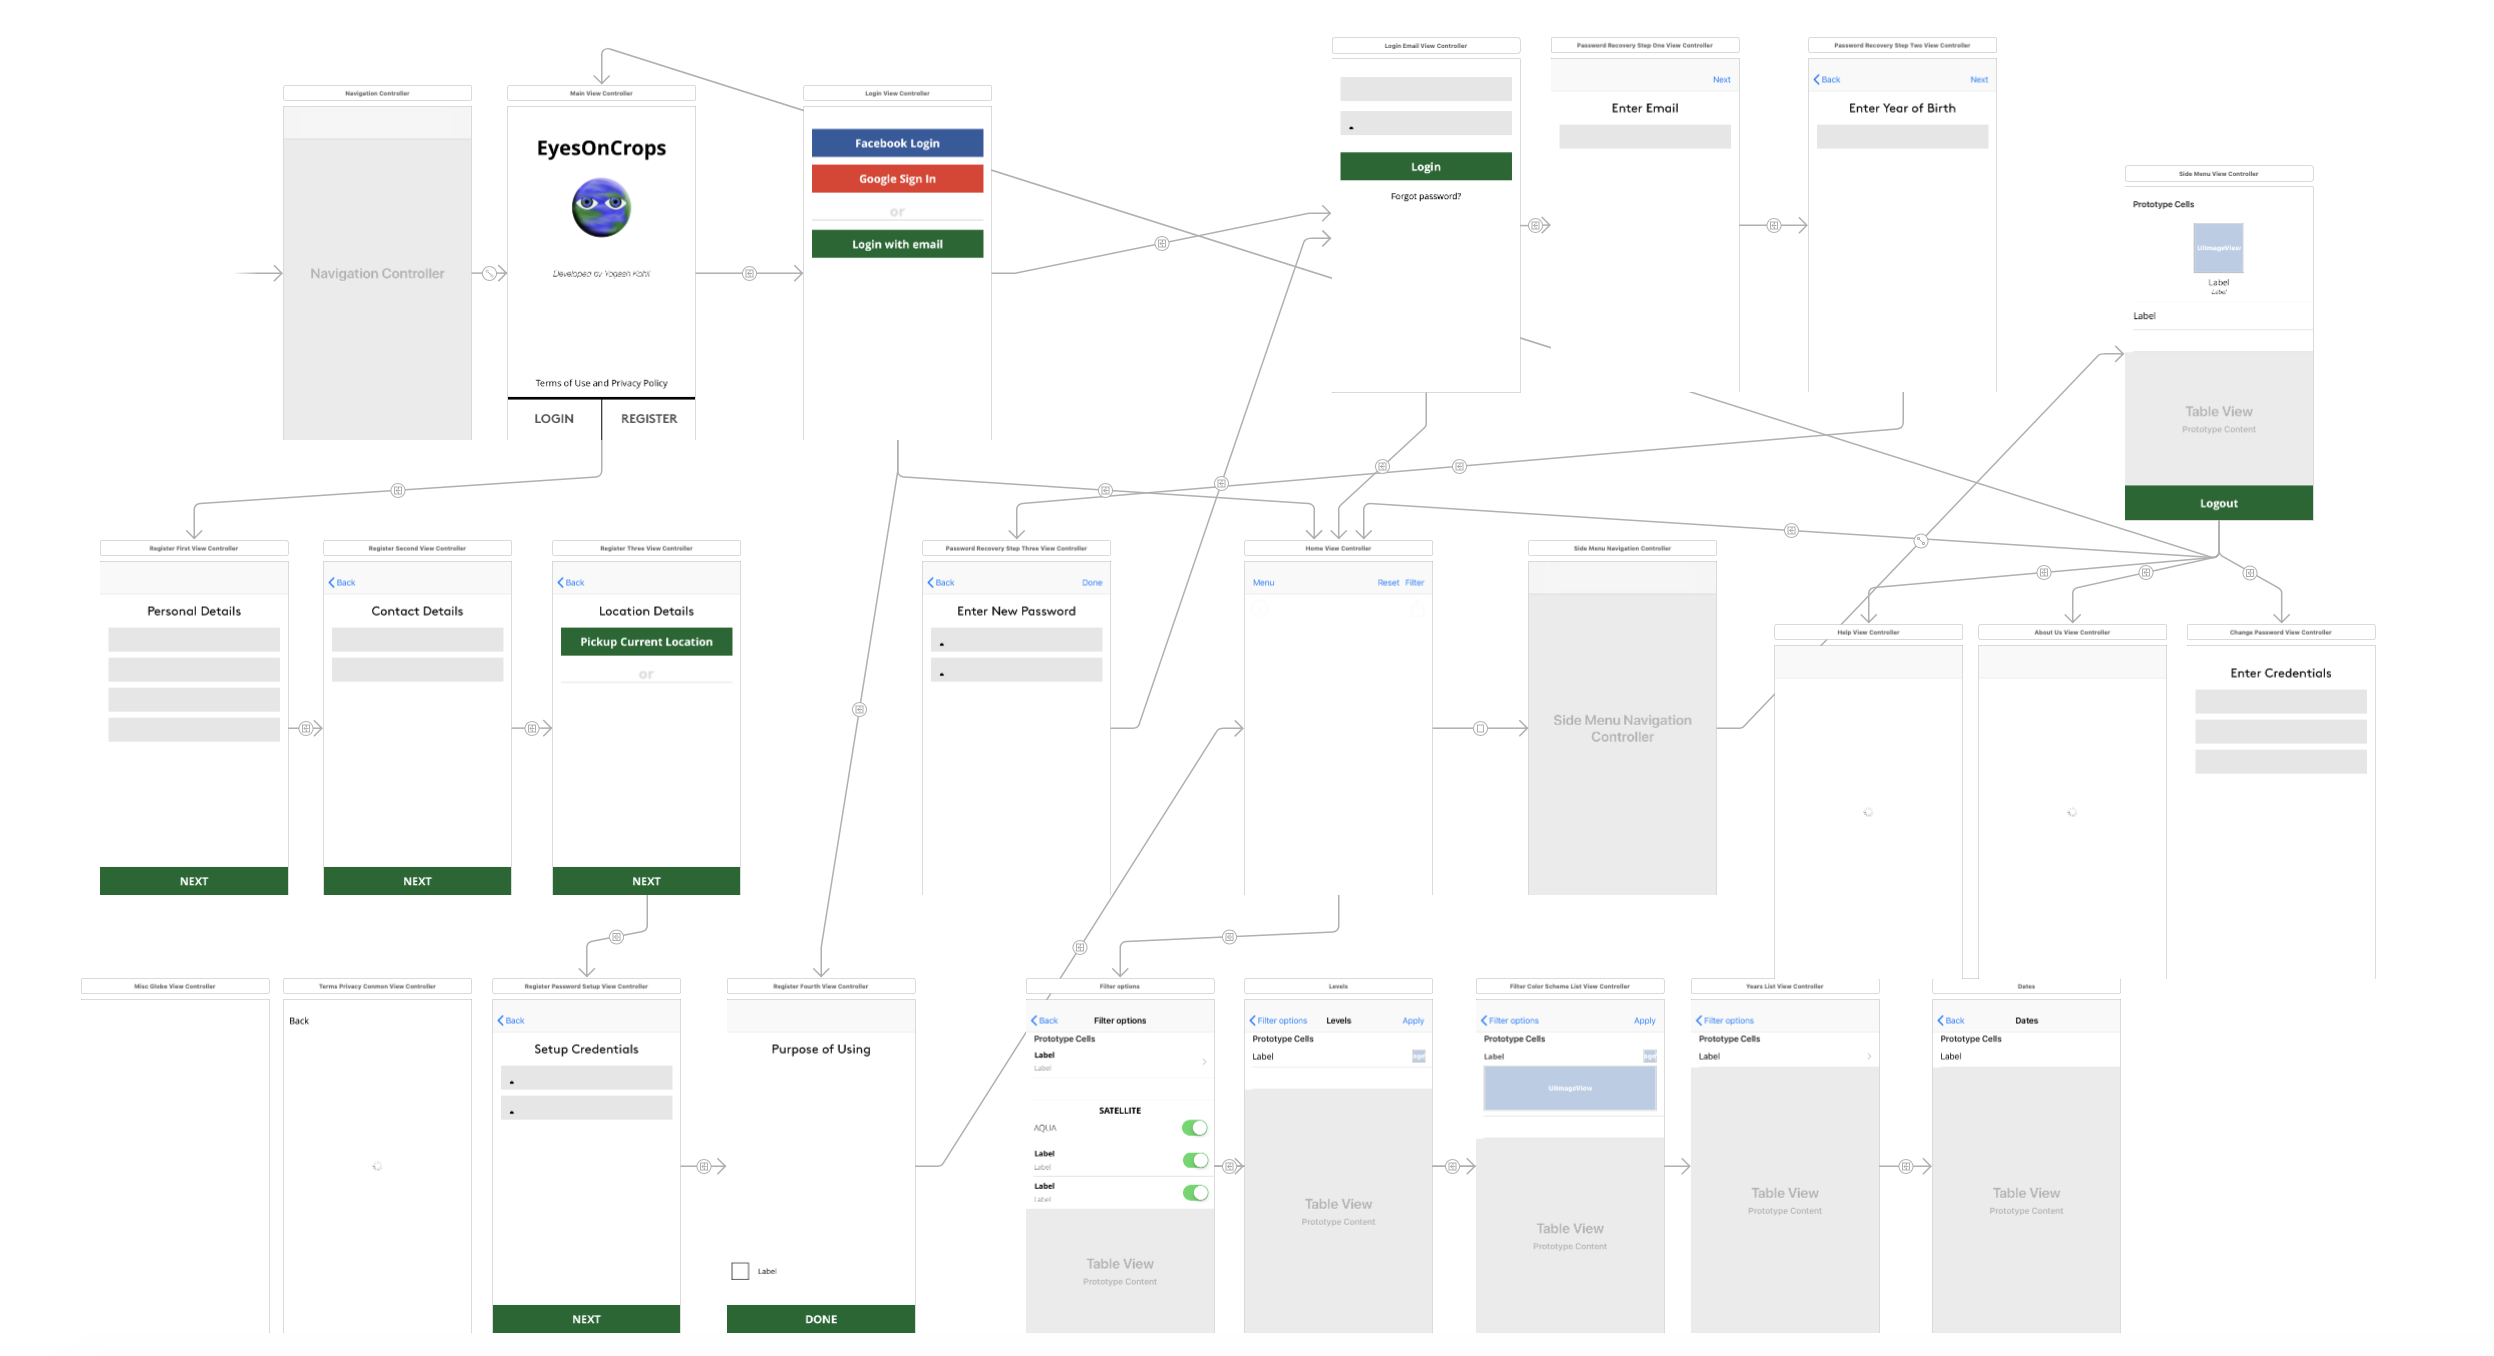
\includegraphics[width=\linewidth]{figures/ch4/storyboard_final.png}
            \caption{\label{fig:wireframe_3} Storyboard of the app}
    \end{figure}
    
\subsection{Mobile App screens and their significance}

\subsubsection{Sign-up via Email}

Sign up process is a one time process which enables you to enter the application out of the blue. It likewise gives us the chance to include the client in our database for future logins and additionally the record.

Sign up via email process consists of 5 screens which are listed below:-

\newpage

\begin{itemize}

    \item Personal details
    
    \begin{figure}[H]
            \centering
            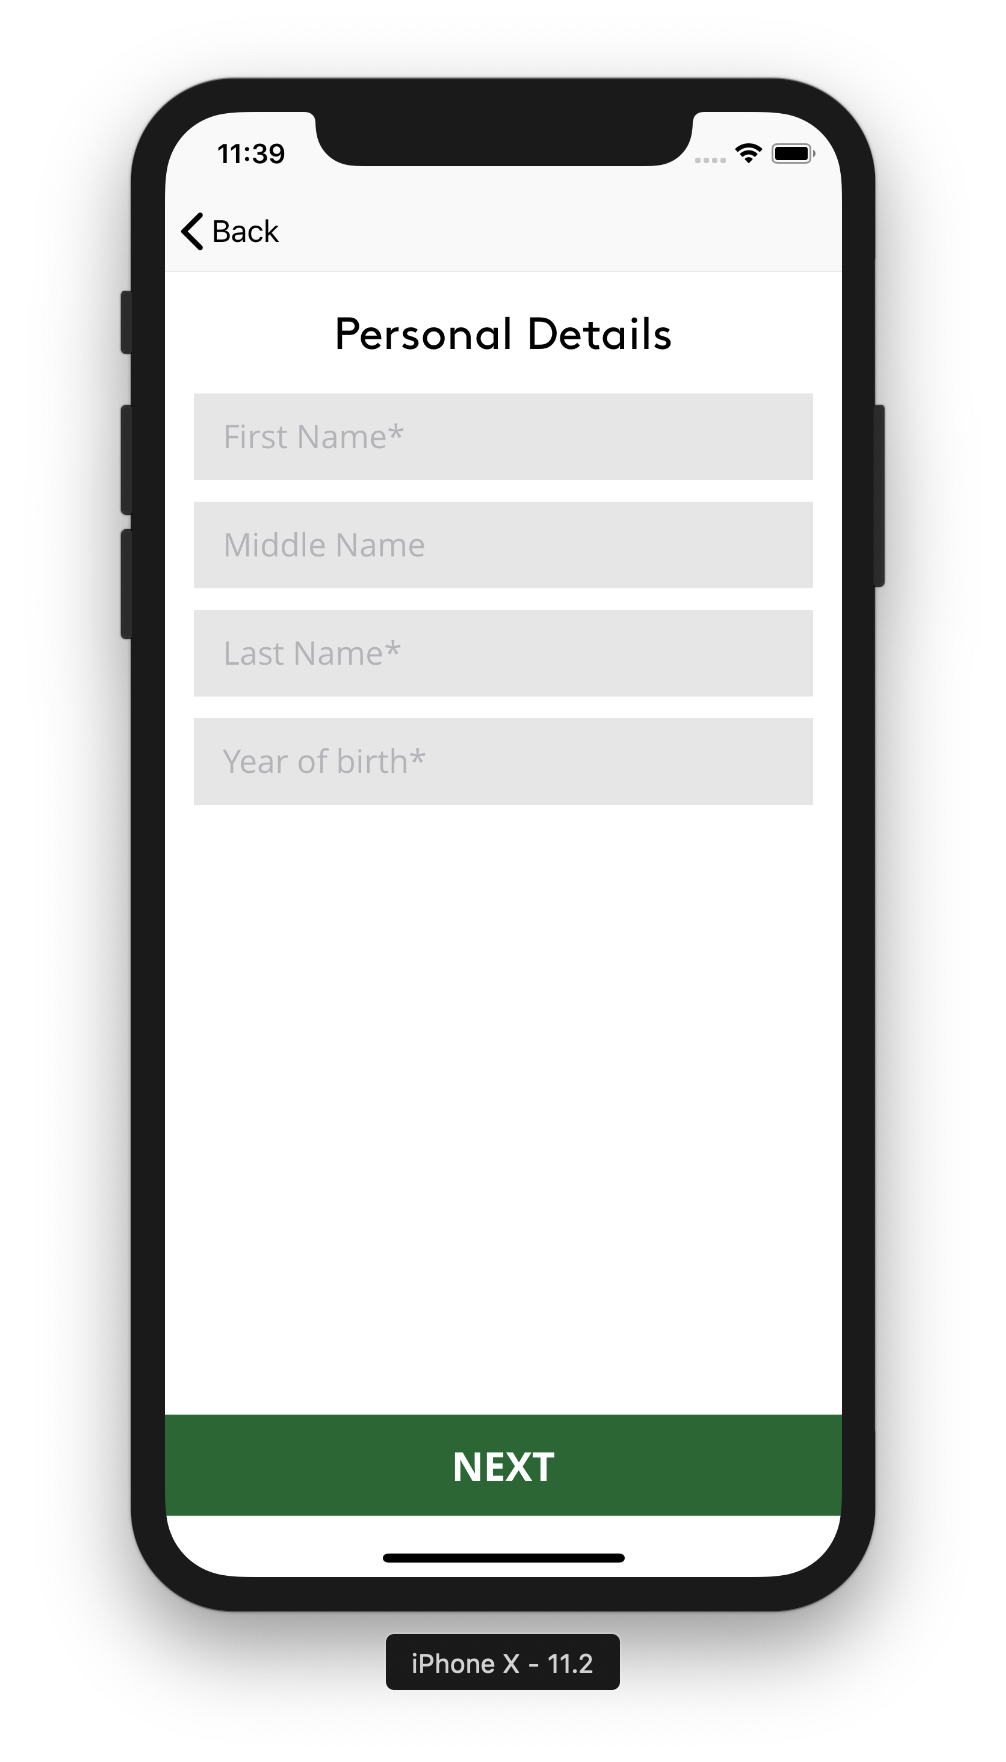
\includegraphics[width=0.4\linewidth]{figures/ch2/register_personal.png}
            \caption{\label{fig:wireframe_3} Register Part-I Personal detail screen}
    \end{figure}
    
    Here in the figure 4.2, mandatory fields are First name, Last name and year of birth where as we have kept middle name as an optional because not everyone has one. \\
    
    UIPickerView is used for selection of year of birth, According to Apple's documentation, UIPickerView is a view that uses a spinning-wheel or slot-machine metaphor to show one or more sets of values.
    
    Figure 4.3 shows the image of the pickerview designed in the app.
    
    \begin{figure}[H]
            \centering
            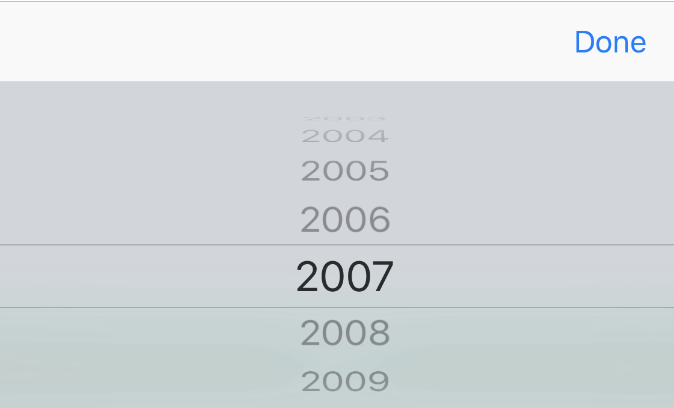
\includegraphics[width=0.4\linewidth]{figures/ch4/pickerview.png}
            \caption{\label{fig:wireframe_3} UIPickerView for year selection}
    \end{figure}
    
    \newpage
    
    \item Contact details
    
    \begin{figure}[H]
            \centering
            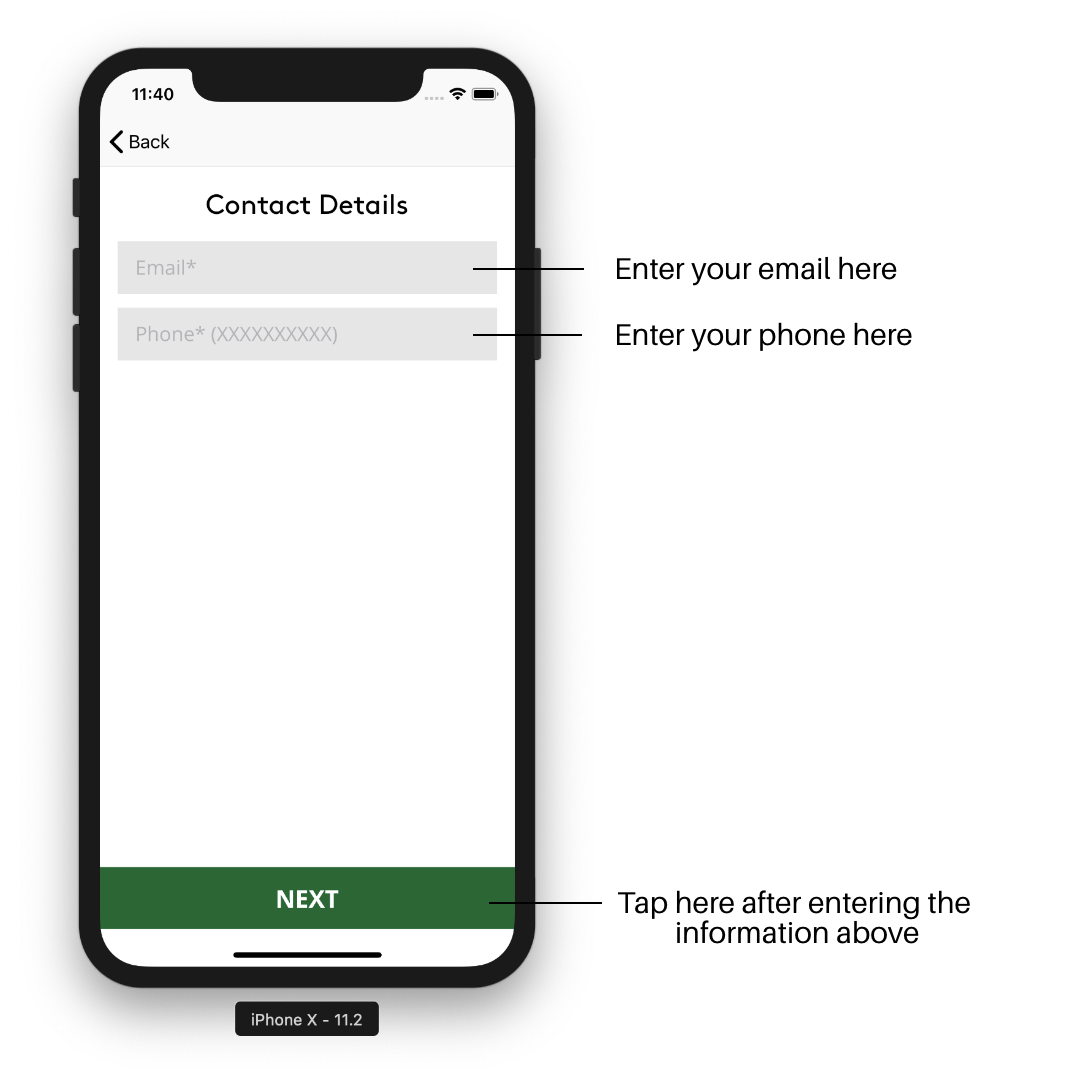
\includegraphics[width=0.5\linewidth]{figures/ch2/register_contact.png}
            \caption{\label{fig:wireframe_3} Register Part-II Contact detail screen}
    \end{figure}
    
    Figure 4.3 represents contact detail screen in which both the fields i.e Email and Phone are mandatory for record purpose and to avoid fake entries. User with unique email and phone can register only once. It's a good point to note that both the fields have been verified syntactically here.
    
    \newpage
  
    \item Location details
    
    \begin{figure}[H]
            \centering
            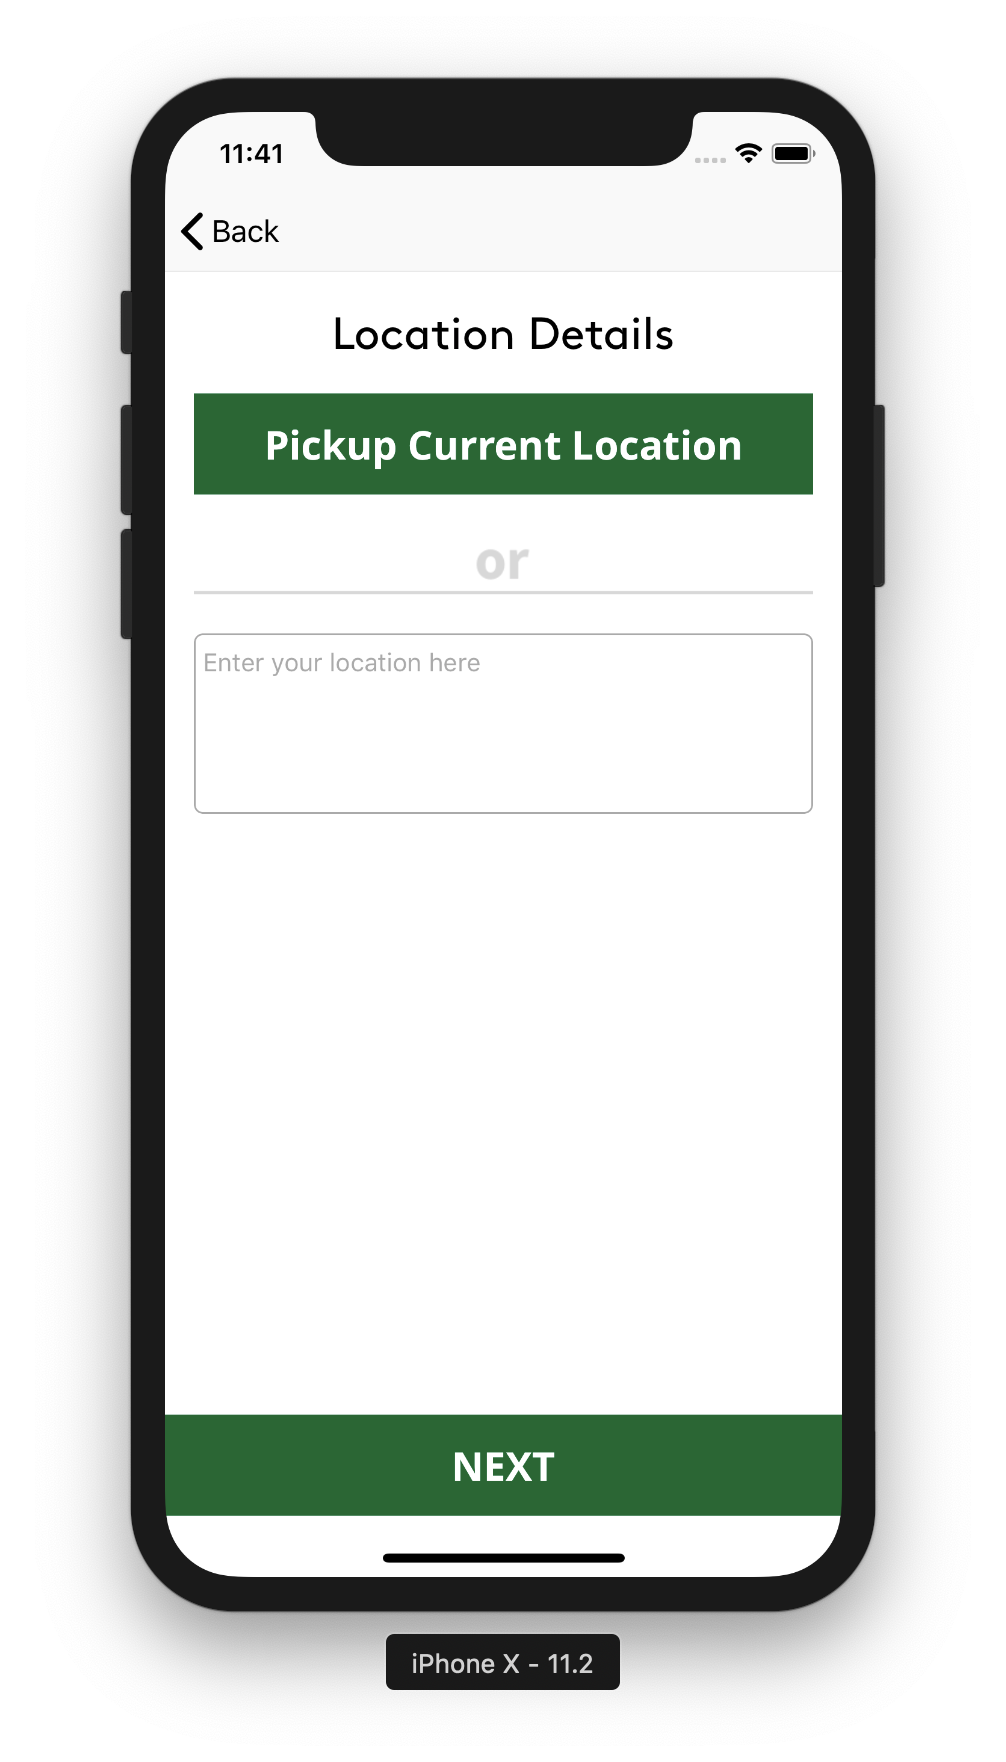
\includegraphics[width=0.5\linewidth]{figures/ch2/register_location.png}
            \caption{\label{fig:wireframe_3} Register Part-III Location detail screen}
    \end{figure}
    
    This screen makes use of Apple's Core Location framework which allows developers to obtain current geographic location of device.
    
    In this screen, user has two possible choices for entering his location, he can enter the area physically or can simply tap on pickup current area which will eventually get the present location and display it in text area showed. Despite everything he can still alter the area if he wants to.
    
    \newpage
    
    \item Setup Credentials
    
    \begin{figure}[H]
            \centering
            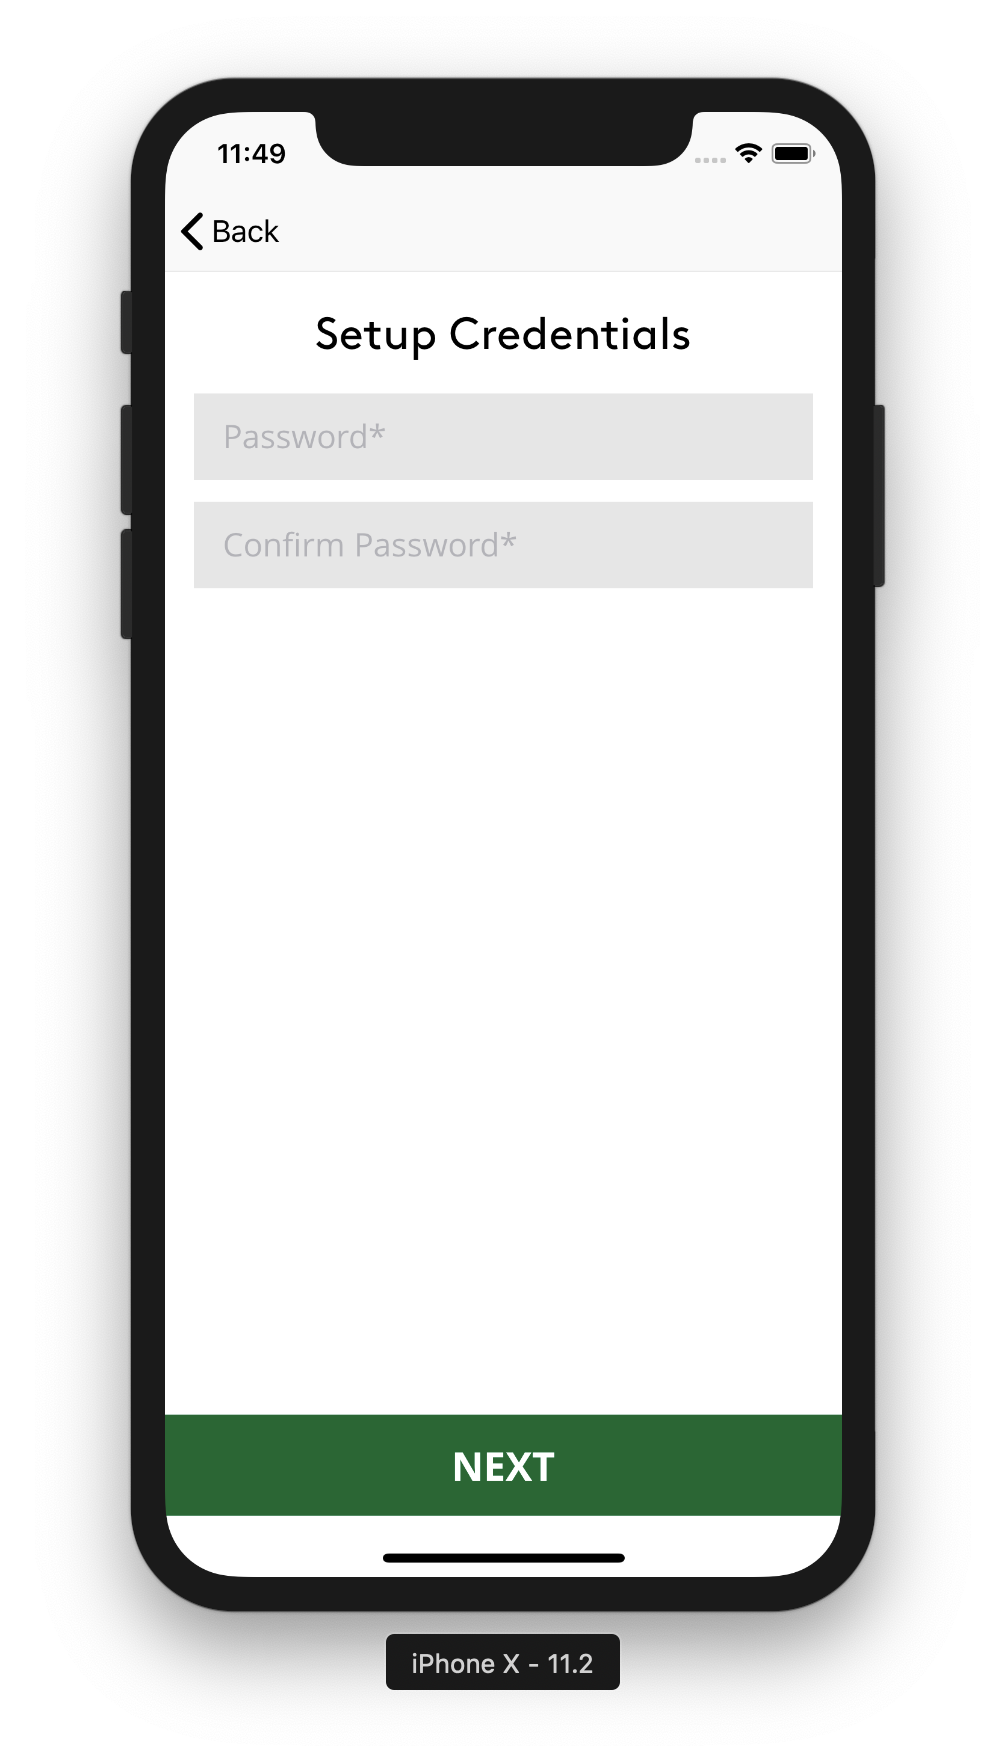
\includegraphics[width=0.5\linewidth]{figures/ch2/credentials_setup.png}
            \caption{\label{fig:wireframe_3} Register Part-IV Credentials setup screen}
    \end{figure}
    
    As you can see in figure 4.6, it allows you to setup password for your secure log in. Point to note here is that minimum length of password has been set 6 digits.
    
    
    \newpage
    
    \item Purpose of using the app
    
     \begin{figure}[H]
            \centering
            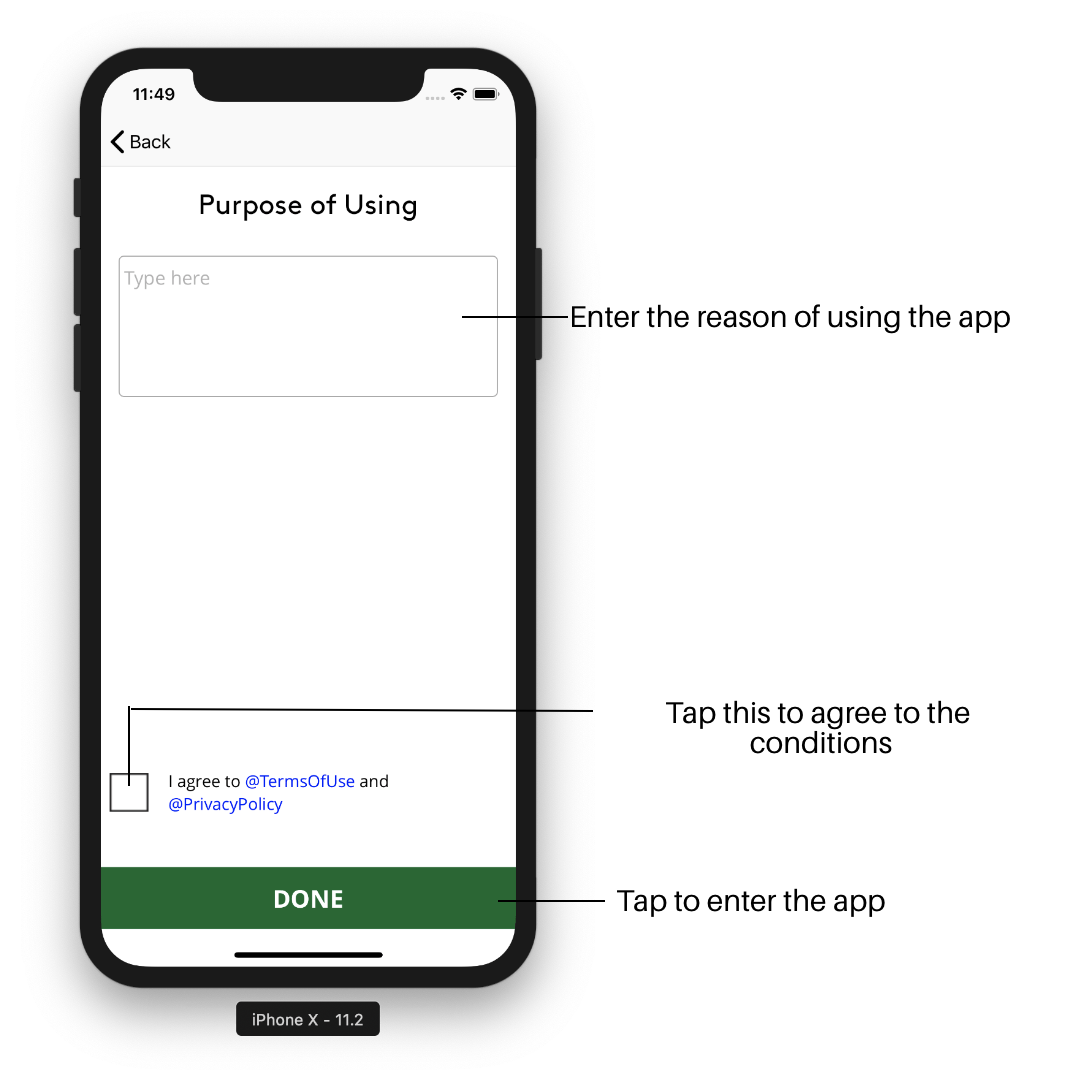
\includegraphics[width=0.5\linewidth]{figures/ch2/purpose_app.png}
            \caption{\label{fig:wireframe_3} Register Part-V Purpose of using the app screen}
    \end{figure}
    
    This screen is really important for us to know what and why people wants to use this app. Moreover, it has additional check mark for privacy policy and terms of use to which every user must agree before going further. It also protects us from some bot attack.
    
    \newpage
 
\end{itemize}


\subsubsection{Login process}

User can log in in the app via certain ways:-

\begin{itemize}
    \item Social Login
    
    Login functionality has been provided using social platforms mentioned below :-
    
    \begin{itemize}
        \item Facebook Login
        
       The Facebook \gls{sdk} for \gls{iOS} provides developers to integrate a plugin through which user can log in with their Facebook account.
       
       Figure 4.8 shows the pop up alert which comes after tapping on Facebook login button and 4.9 shows the screens when user opts for Facebook log in after clicking continue in fig 4.8
       
      \begin{figure}[!htb]
        \begin{minipage}{0.5\textwidth}
            \centering
            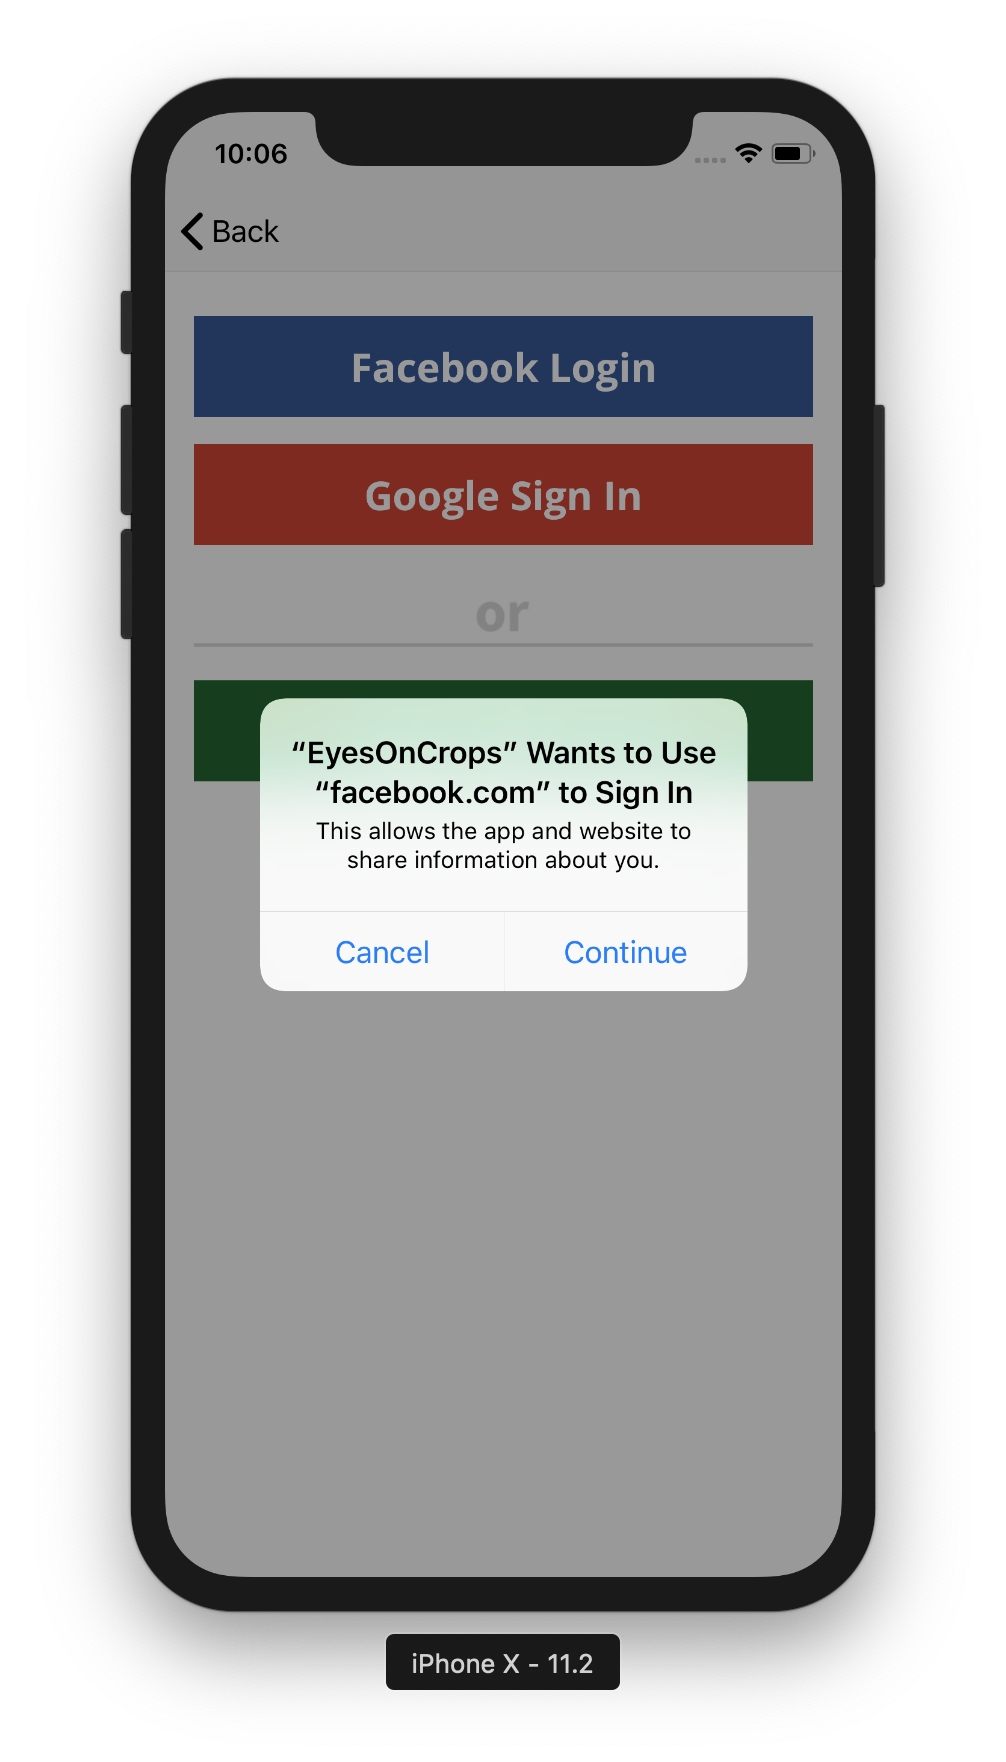
\includegraphics[width=0.8\linewidth]{figures/ch4/facebook_1.png}
            \caption{Facebook log in Part-I}\label{Fig:facebook_part_1}
        \end{minipage}\hfill
        \begin{minipage}{0.5\textwidth}
            \centering
            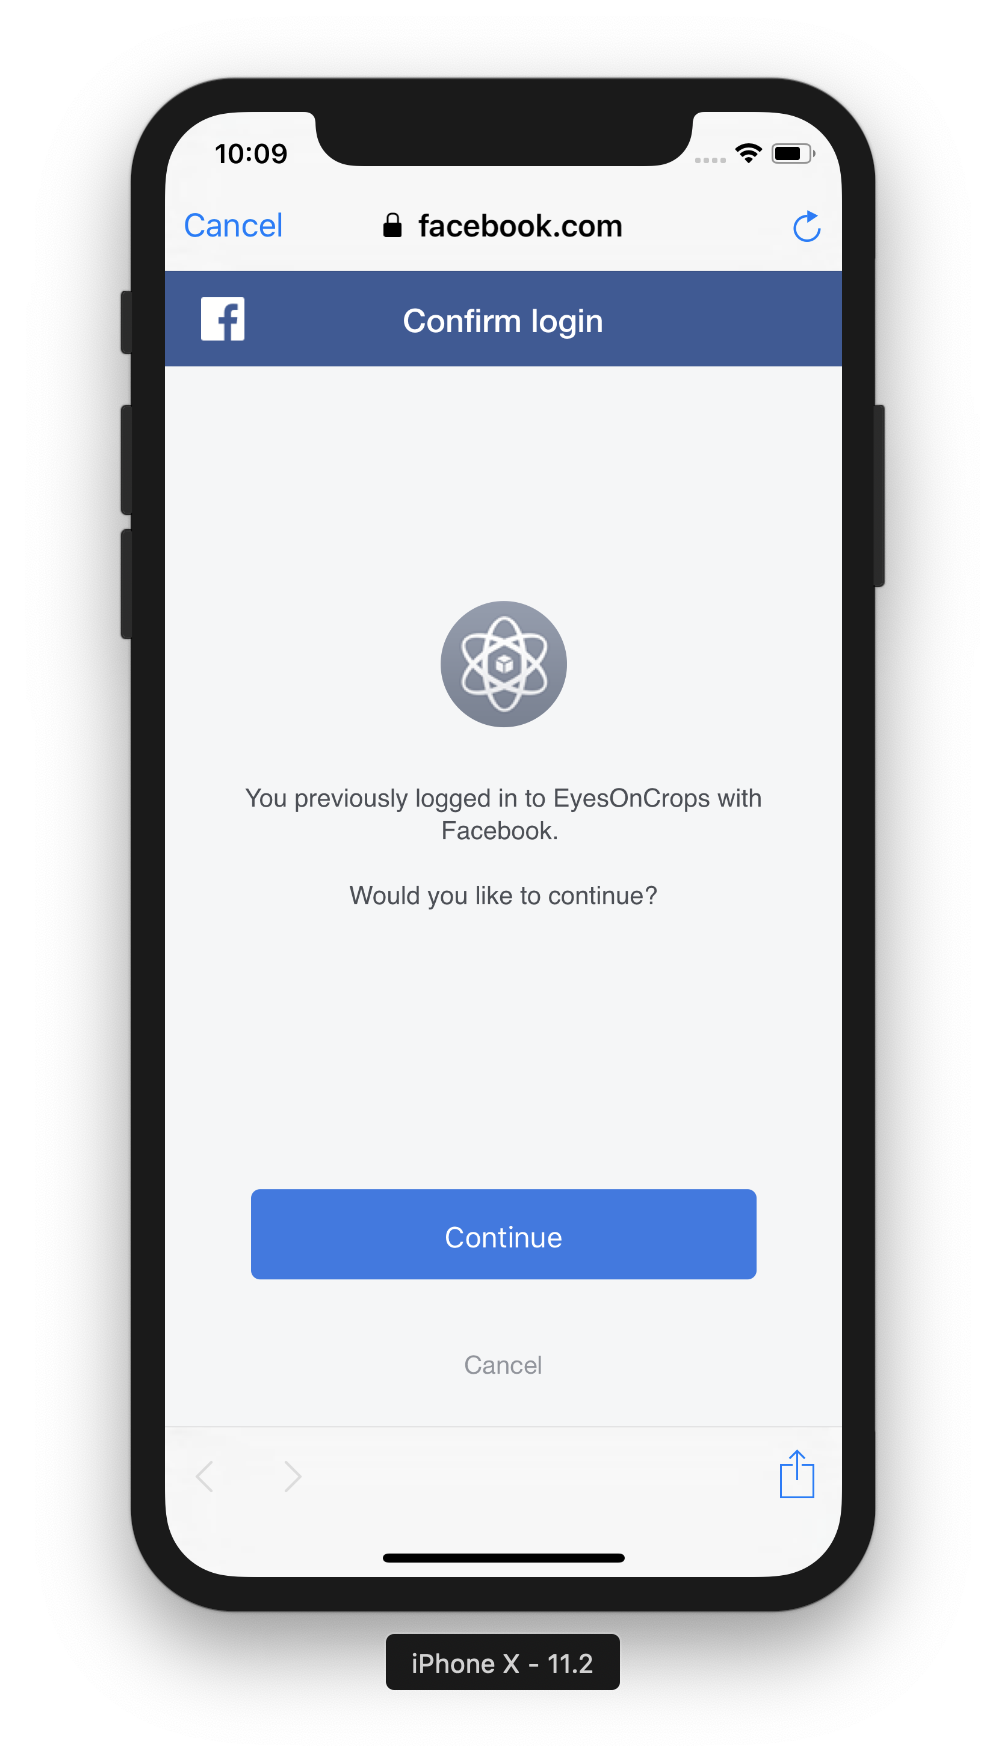
\includegraphics[width=0.8\linewidth]{figures/ch4/facebook_2.png}
            \caption{Facebook log in Part-II}\label{Fig:facebook_part_2}
        \end{minipage}
    \end{figure}
    
        As you can see in fig 4.9, user doesn't have to enter his Facebook id and password every time, it's a one time process, the \gls{sdk} helps developers to remember the credentials used previously they logged in on the app.
        
        \newpage
       
        \item Google Sign in
        
        User can also log in through their Gmail account by tapping on Google sign in button in the fig 4.10 if they don't have Facebook account or vice-verse.
        I have used Google's \gls{api} for Sign in to \gls{iOS} devices to create this functionality in the app. \\
        
        Figure 4.10 and 4.11 shows Google \gls{sdk} sign in process.
        
        \begin{figure}[!htb]
        \begin{minipage}{0.5\textwidth}
            \centering
            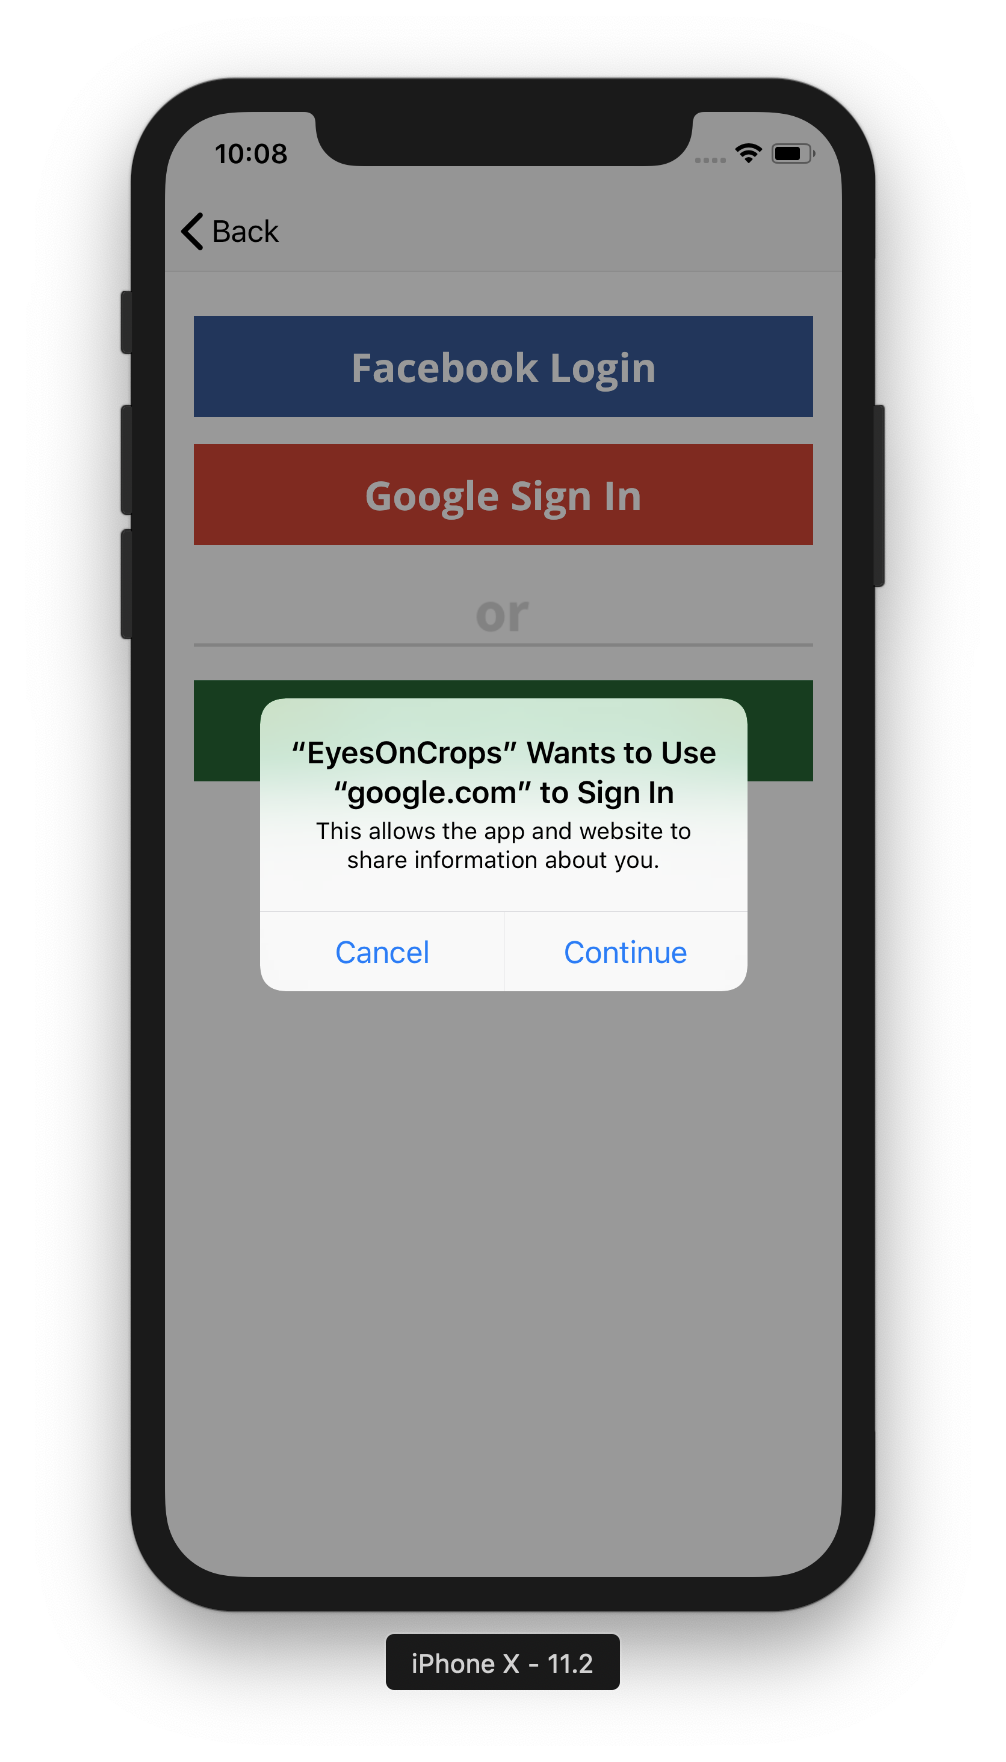
\includegraphics[width=0.8\linewidth]{figures/ch4/google_1.png}
            \caption{Google sign in Part-I}\label{Fig:google_part_1}
        \end{minipage}\hfill
        \begin{minipage}{0.5\textwidth}
            \centering
            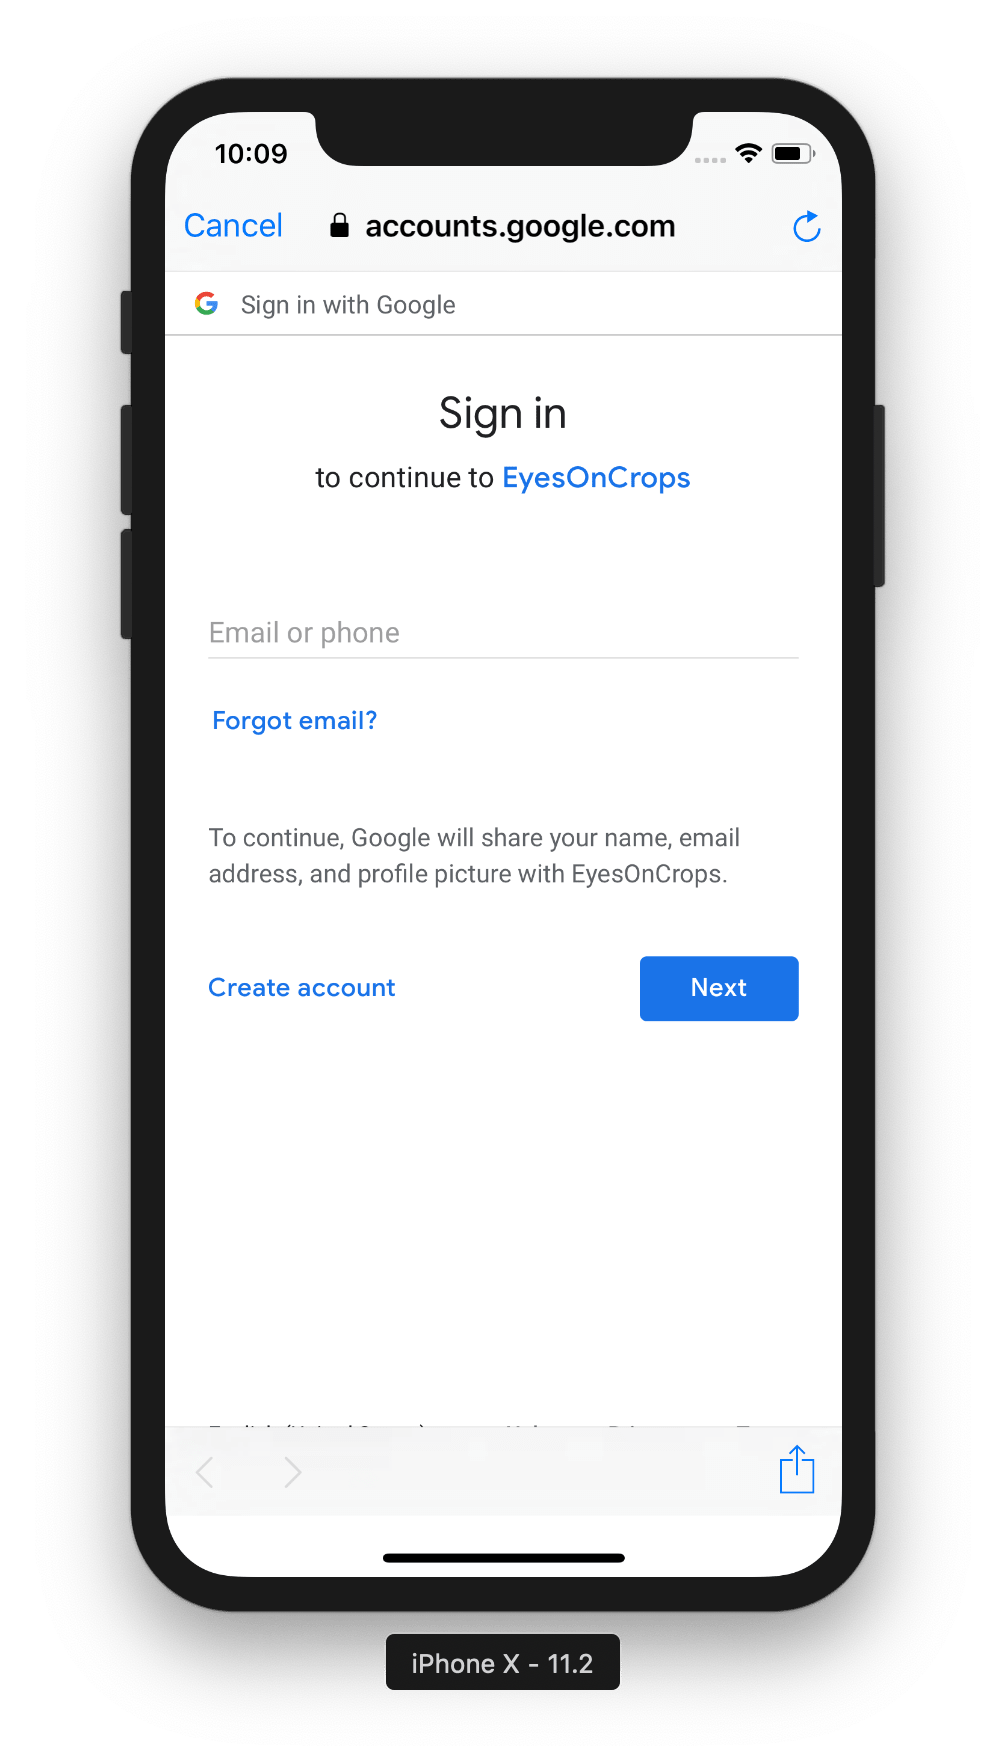
\includegraphics[width=0.8\linewidth]{figures/ch4/google_2.png}
            \caption{Google sign in Part-II}\label{Fig:google_part_2}
        \end{minipage}
    \end{figure}
        
    \end{itemize}
    
    \newpage
    
    \item Login via email
    
    Those users who have registered via email can utilize the functionality of log in via email.
    
    They will be required to enter valid email and password to do so.
    
    Figure 4.12 shows the login with email screen.
    
    \begin{figure}[H]
            \centering
            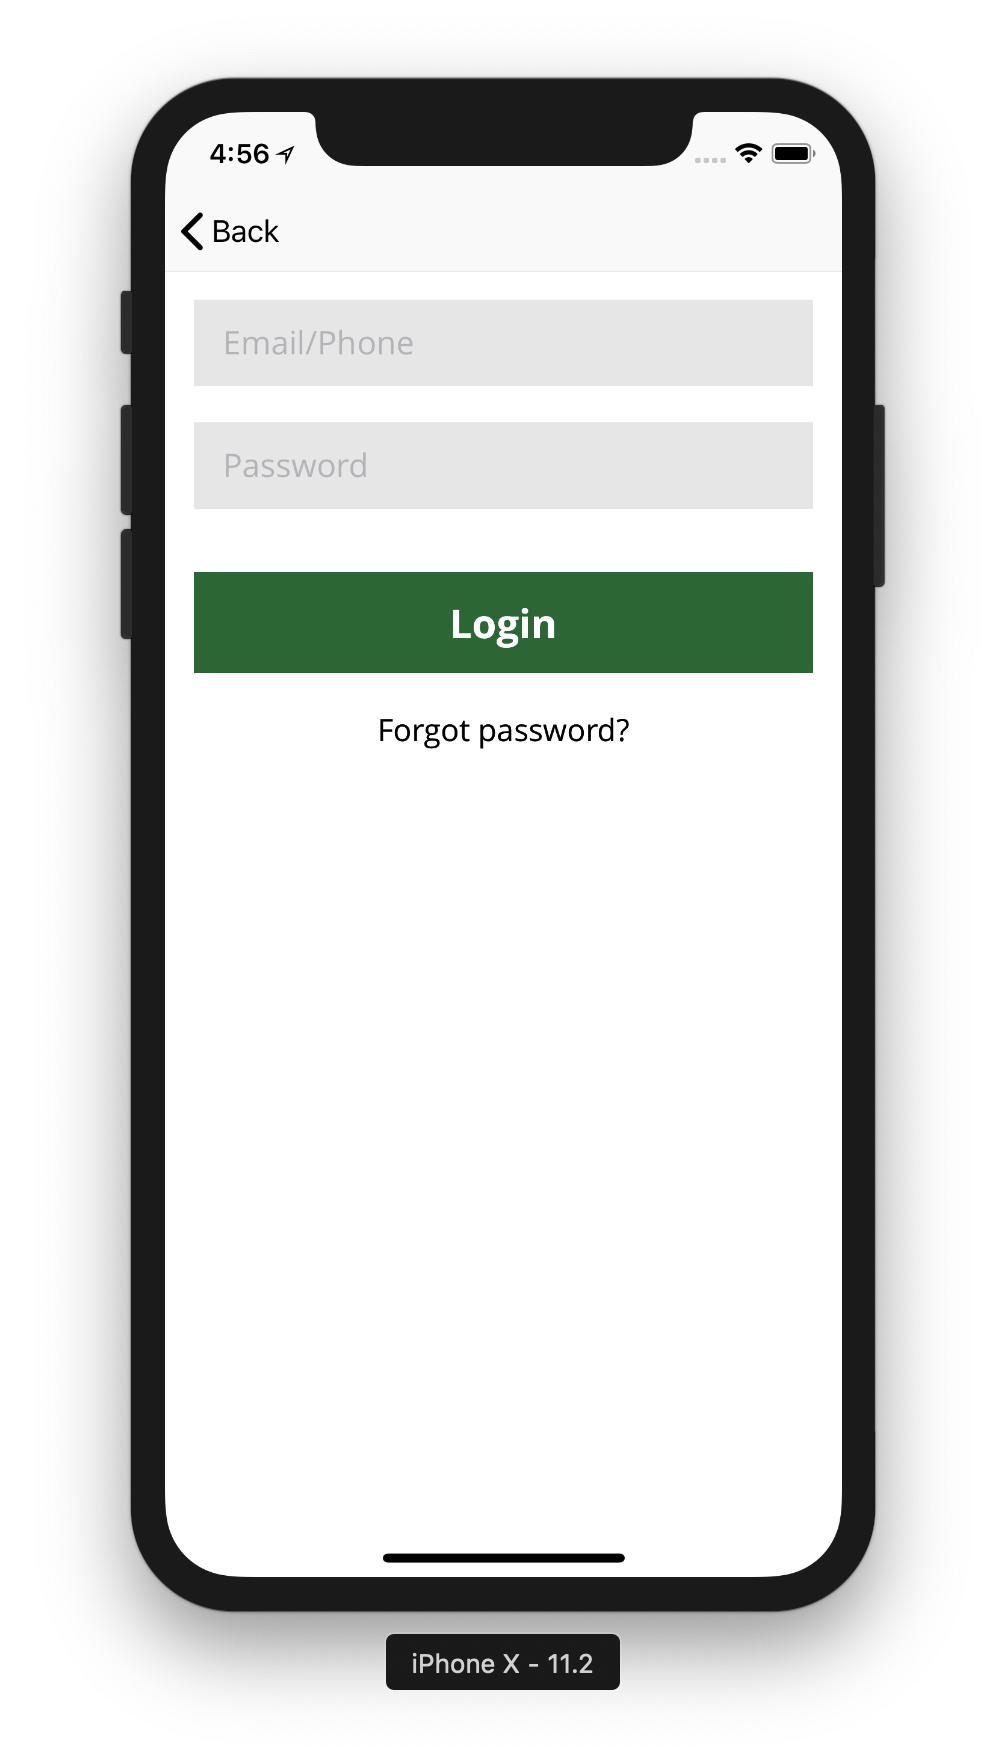
\includegraphics[width=0.5\linewidth]{figures/ch2/login_email.png}
            \caption{\label{fig:wireframe_3} Login via email}
    \end{figure}
    
    
    Also, if ever user has forgot his password, he can tap on forgot password button in fig 4.12 and follow the certain steps to change his password. \\
    
    \newpage
    
    \textbf{Password recovery} screens and their significance are as follows :-
    
    \begin{itemize}
        \item Email verification screen
        
        \begin{figure}[H]
            \centering
            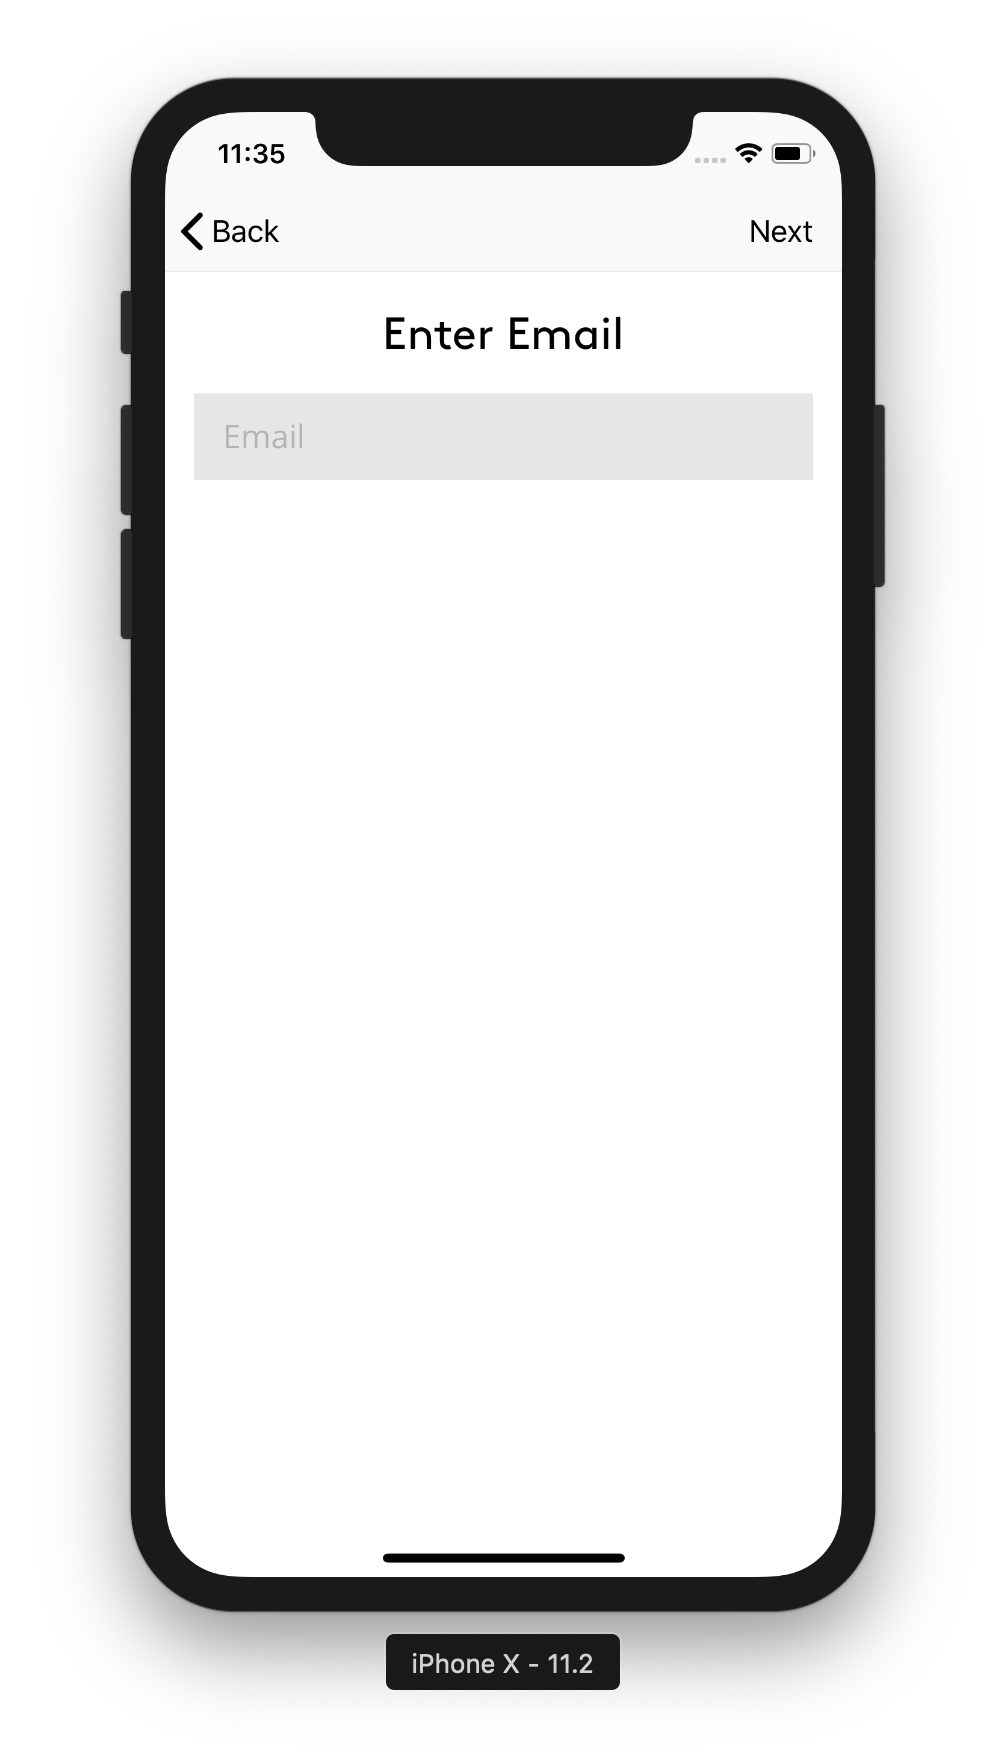
\includegraphics[width=0.5\linewidth]{figures/ch4/pass_recovery_1.png}
            \caption{\label{fig:pass_recovery_1} Password Recovery Part-I - Email verification}
        \end{figure}
    
    First part of the password recovery is to check if the user exist with the email he entered in the fig 4.13. If yes, then take him to next screen else show him the alert saying that record does not exist with this email.
    
     \newpage
    
     \item Year of birth verification screen
        
        \begin{figure}[H]
            \centering
            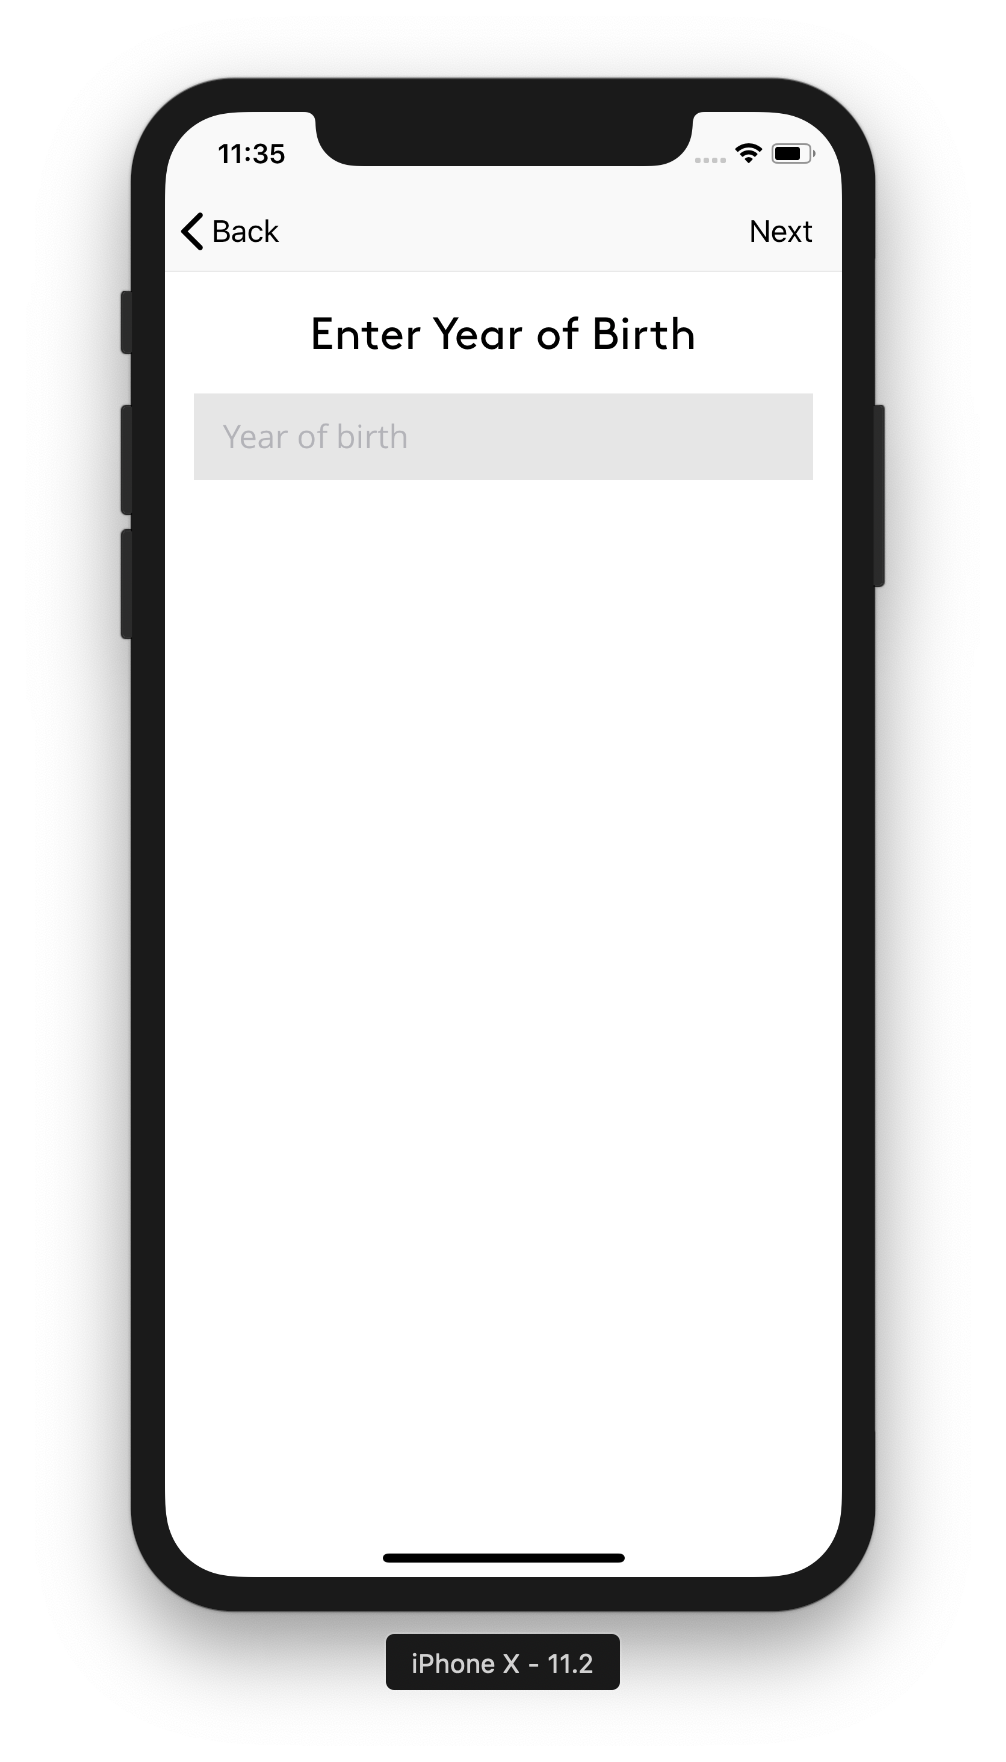
\includegraphics[width=0.5\linewidth]{figures/ch4/pass_recovery_2.png}
            \caption{\label{fig:pass_recovery_1} Password Recovery Part-II - Year of birth verification}
    \end{figure}
    
    This screen is to make this process more secure by asking user his year of birth. It must match the year of birth he entered in registering via email process.
    If this matches, then allow him to change his password.
    
     \newpage
    
     \item Change credentials screen
        
        \begin{figure}[H]
            \centering
            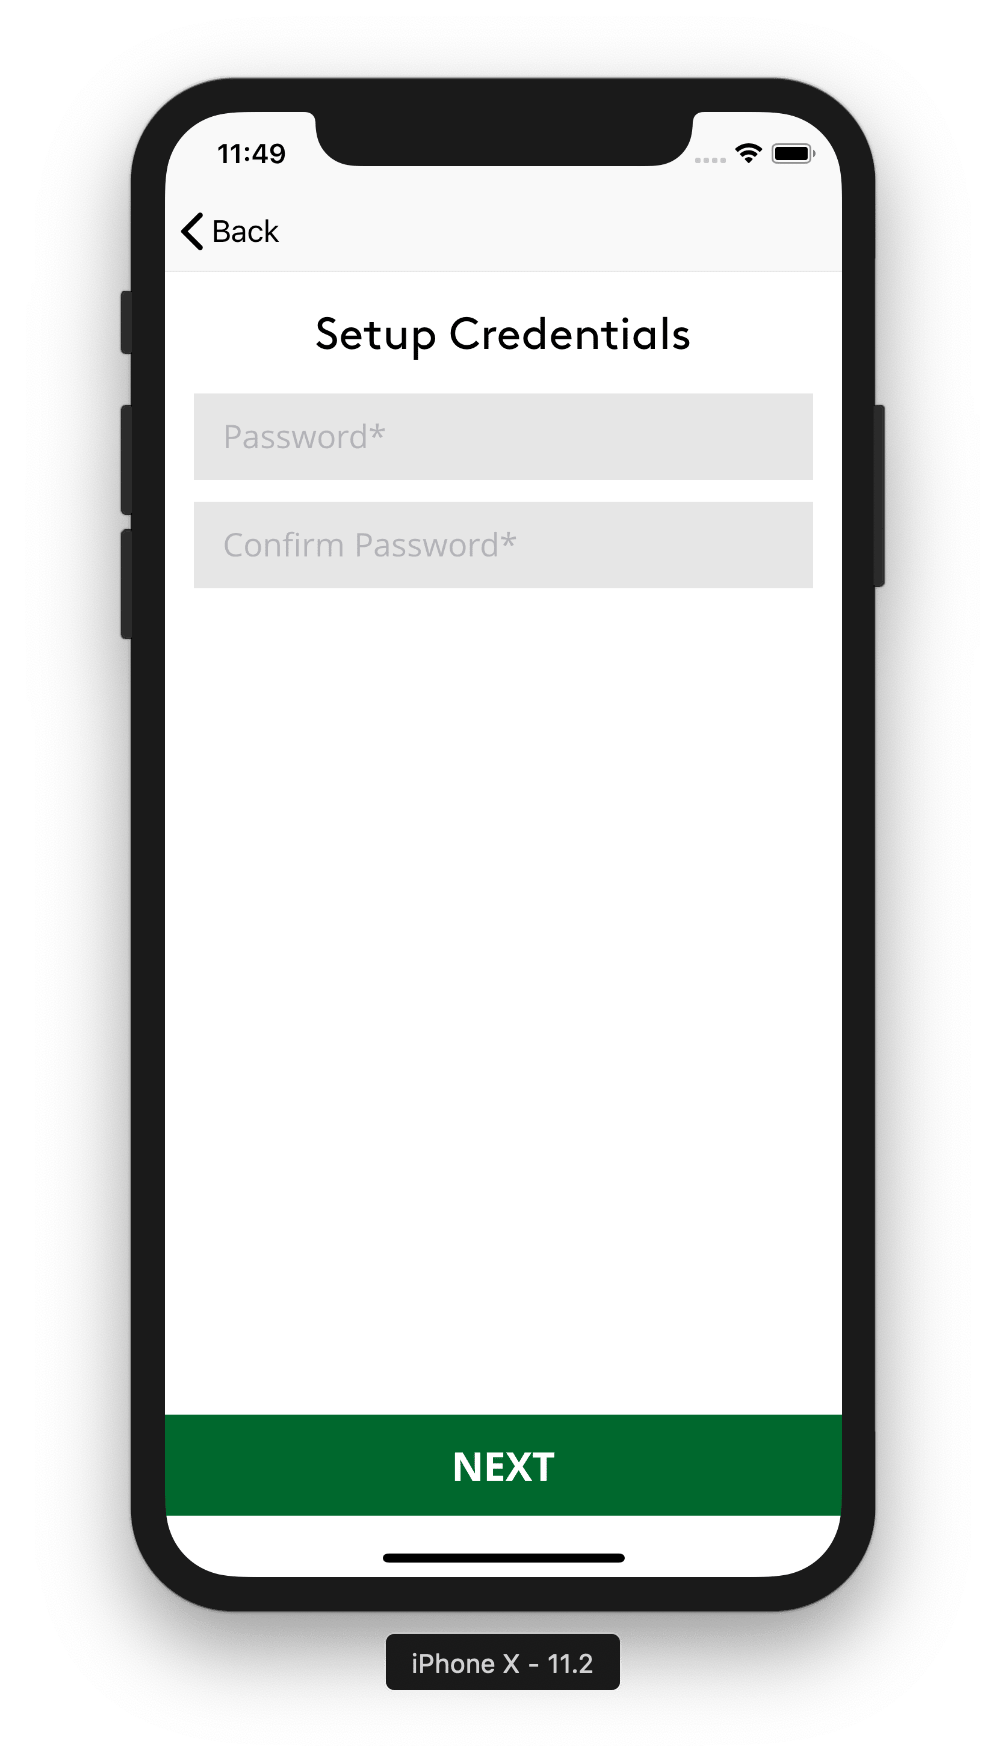
\includegraphics[width=0.5\linewidth]{figures/ch4/pass_recovery_3.png}
            \caption{\label{fig:pass_recovery_1} Password Recovery Part-III- Change credentials screen}
        \end{figure}
    
    Now, this screen enables you to change your password so that you can log in again and enjoy the app.
    
     \newpage
        
    \end{itemize}
    
\end{itemize}

\subsubsection{Home screen}

This is an essential part of any application. In a context of mobile applications, it's the main screen from which users interact with most options of the application. \\

Home screen has two nature which are :-

    \begin{figure}[!htb]
        \begin{minipage}{0.5\textwidth}
            \centering
            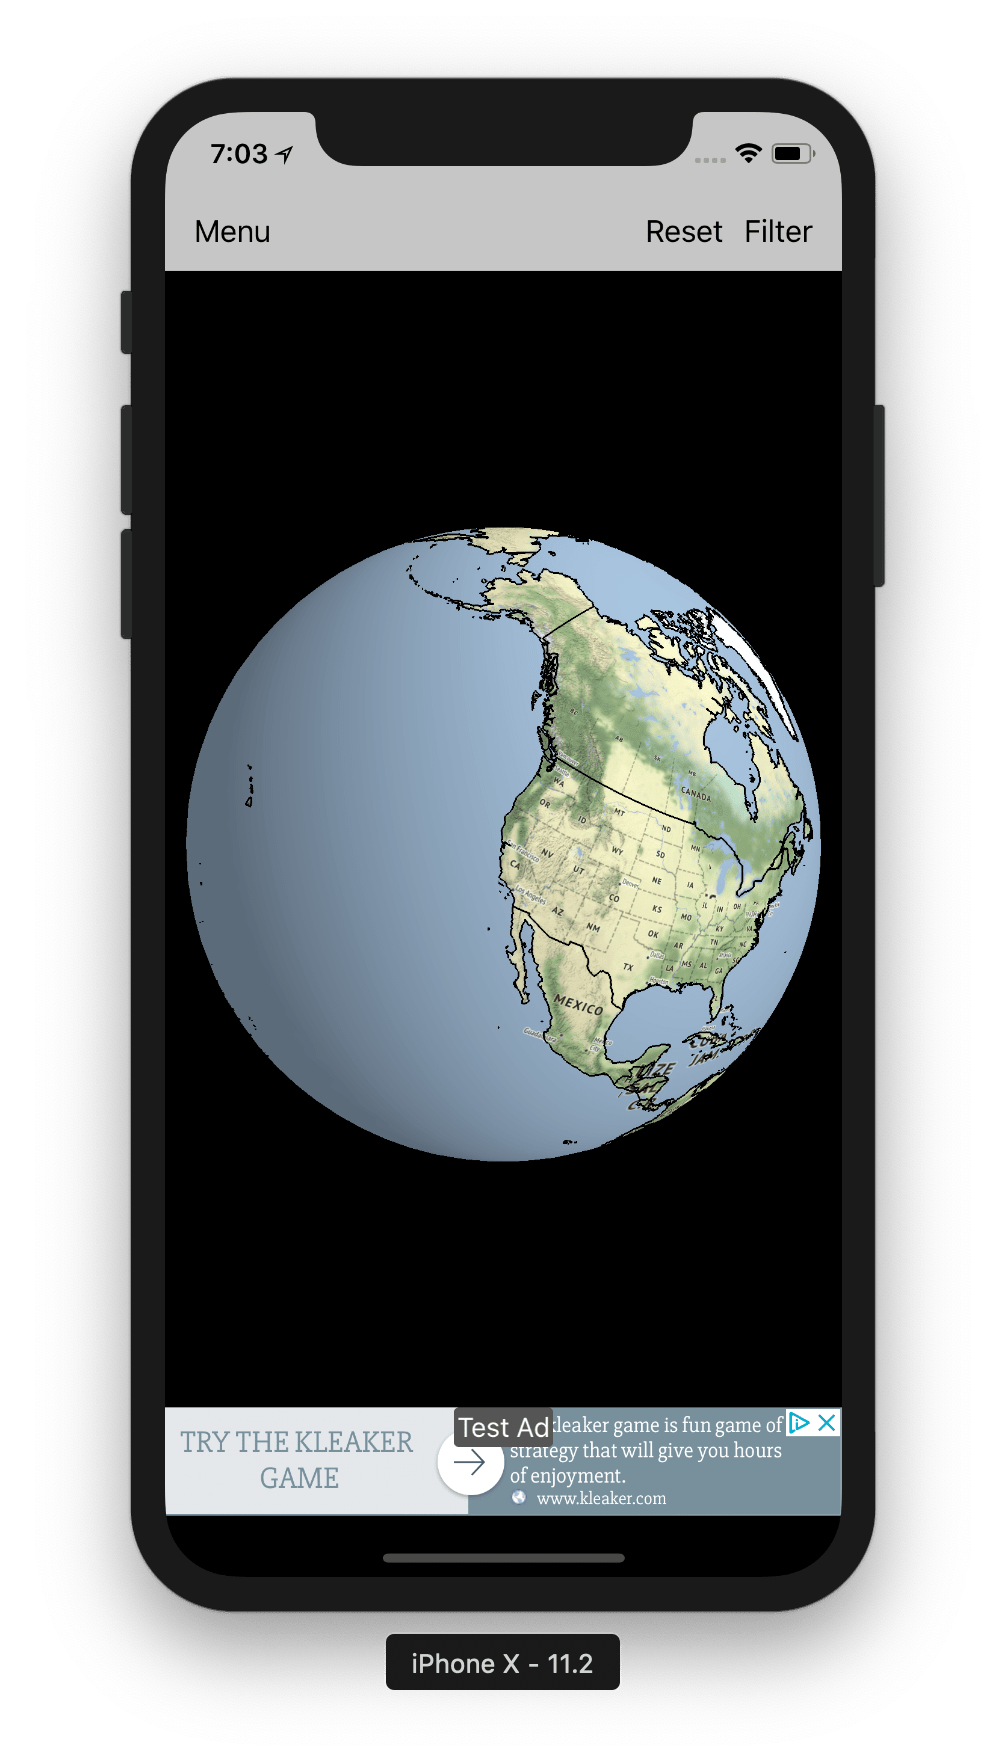
\includegraphics[width=0.8\linewidth]{figures/ch4/home_globe.png}
            \caption{Globe view}\label{Fig:home_globe}
        \end{minipage}\hfill
        \begin{minipage}{0.5\textwidth}
            \centering
            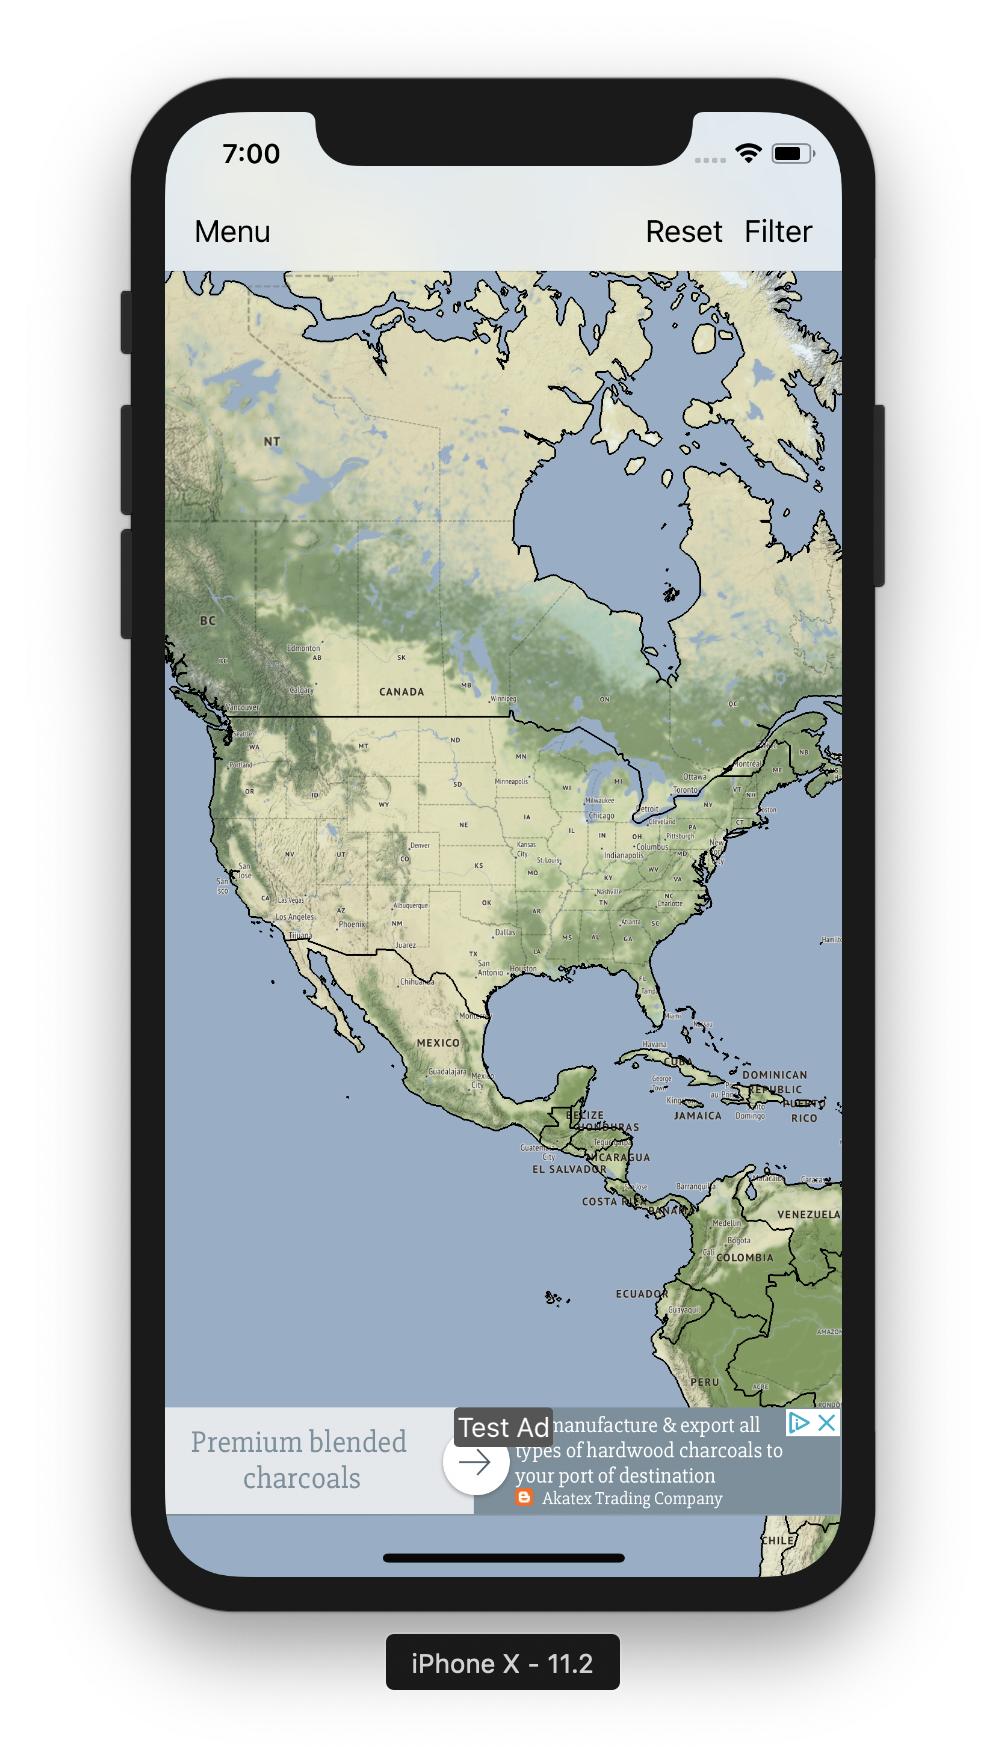
\includegraphics[width=0.8\linewidth]{figures/ch4/home.png}
            \caption{2D Map view}\label{Fig:home_map}
        \end{minipage}
    \end{figure}
    
    It also includes Google Ads at the bottom of the screen. Google AdMob for \gls{iOS} framework has been integrated to achieve this. Google has a lot of different types of ads but the one we have implemented is the banner view.

\newpage

\subsubsection{Sliding Menu}

Sliding menu has been used in the app to make navigation easier for the user. It enables user to visit some of the key screens without any hustle.

Figure 4.16 shows the sliding menu and the options it includes.

    \begin{figure}[H]
            \centering
            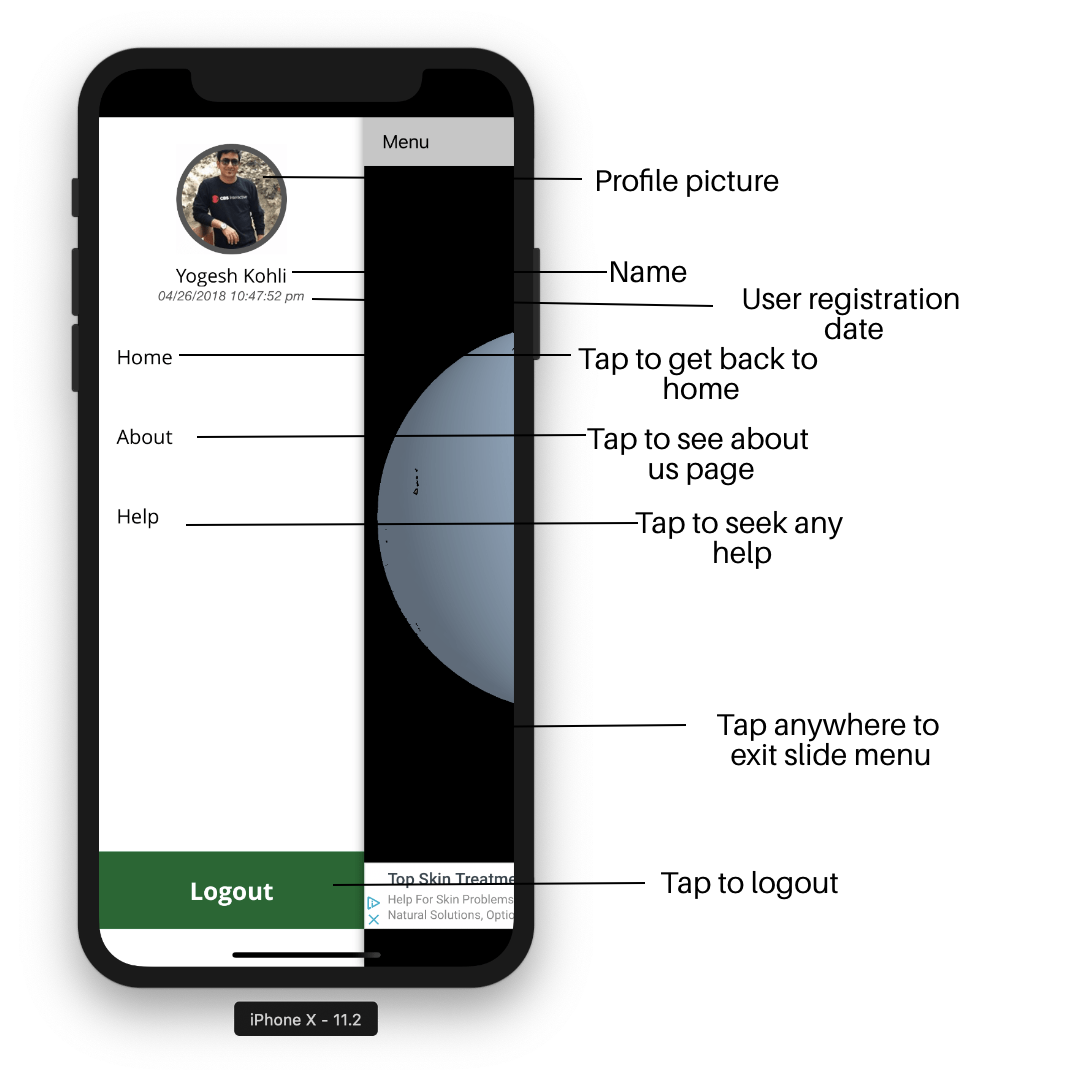
\includegraphics[width=0.5\linewidth]{figures/ch2/side_menu.png}
            \caption{\label{fig:pass_recovery_1} Sliding menu screen}
    \end{figure}

    User can easily navigate to the following :-

    \begin{itemize}
    \item Home \\
    By tapping on home, it takes user to the home i.e landing page.
    
        \item About \\
            The main role of an about us page is to inform user about the organization and its tasks. This is a clear objective that almost all organizations need to satisfy in some form or another.
            
        \begin{figure}[H]
            \centering
            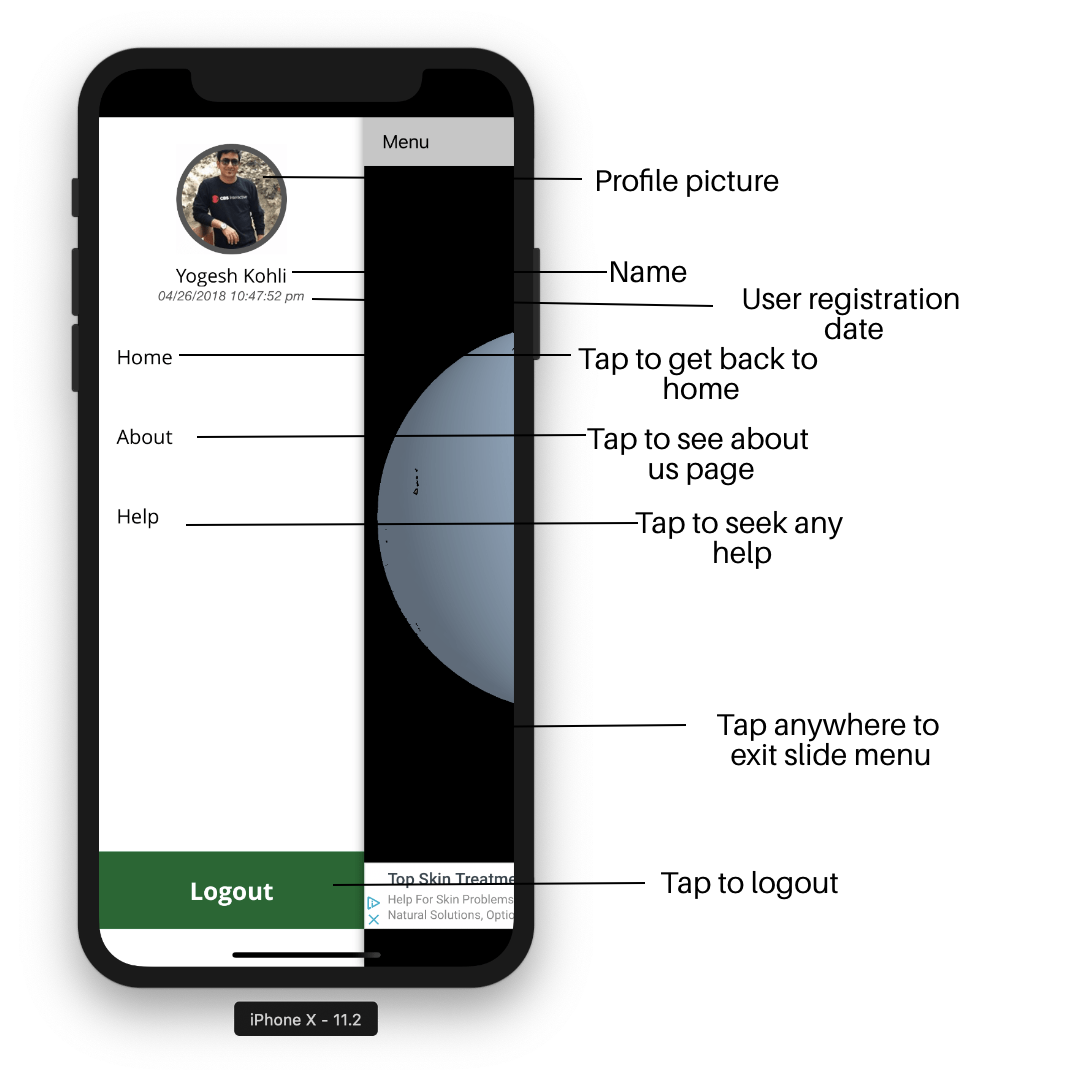
\includegraphics[width=0.5\linewidth]{figures/ch2/side_menu.png}
            \caption{\label{fig:pass_recovery_1} About us screen}
        \end{figure}
        
        \newpage
        
         \item Help \\
            The main reason for keeping help screen in slide menu is to provide user easier access to help in case of any query. He can follow certain steps and contact the developer / organization in case of any difficulties.
            
        \begin{figure}[H]
            \centering
            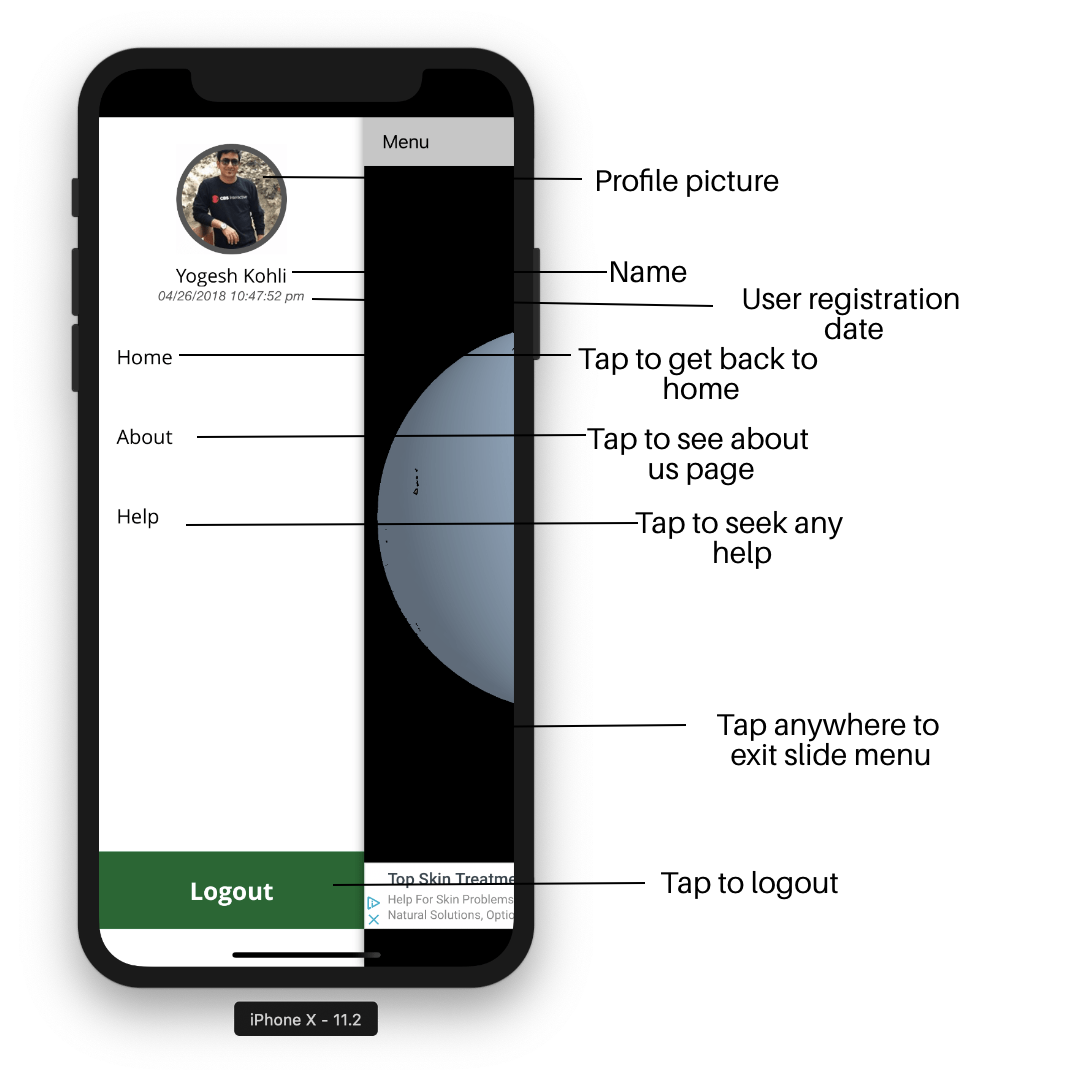
\includegraphics[width=0.5\linewidth]{figures/ch2/side_menu.png}
            \caption{\label{fig:pass_recovery_1} About us screen}
        \end{figure}
        
            \newpage
            
    \end{itemize}

\subsubsection{Filter process}

This is one of the most crucial part of the application which enables user to filter the data according to the needs.

Filtering is being done on various parameters :

%FIGURE MANAGE PROPERLY - CORRECT IMAGES AFTER EDITING - BLURR HERE

\begin{itemize}
    \item \gls{ndvi} or Anomaly data
    
    This feature has been developed to give the user freedom of choosing the type of data he wants to visualize.
    
    A visual toggle - UISwitch has been used for this purpose to enable \gls{ndvi} or anomaly data. By default, \gls{ndvi} is selected. When the user changes the toggle, to make it clear, the text under the heading also changes displaying what is being currently selected.
    
    Both the choices and their text values on selection have been shown in the figures below.
    
    \begin{figure}[!htb]
        \begin{minipage}{0.5\textwidth}
            \centering
            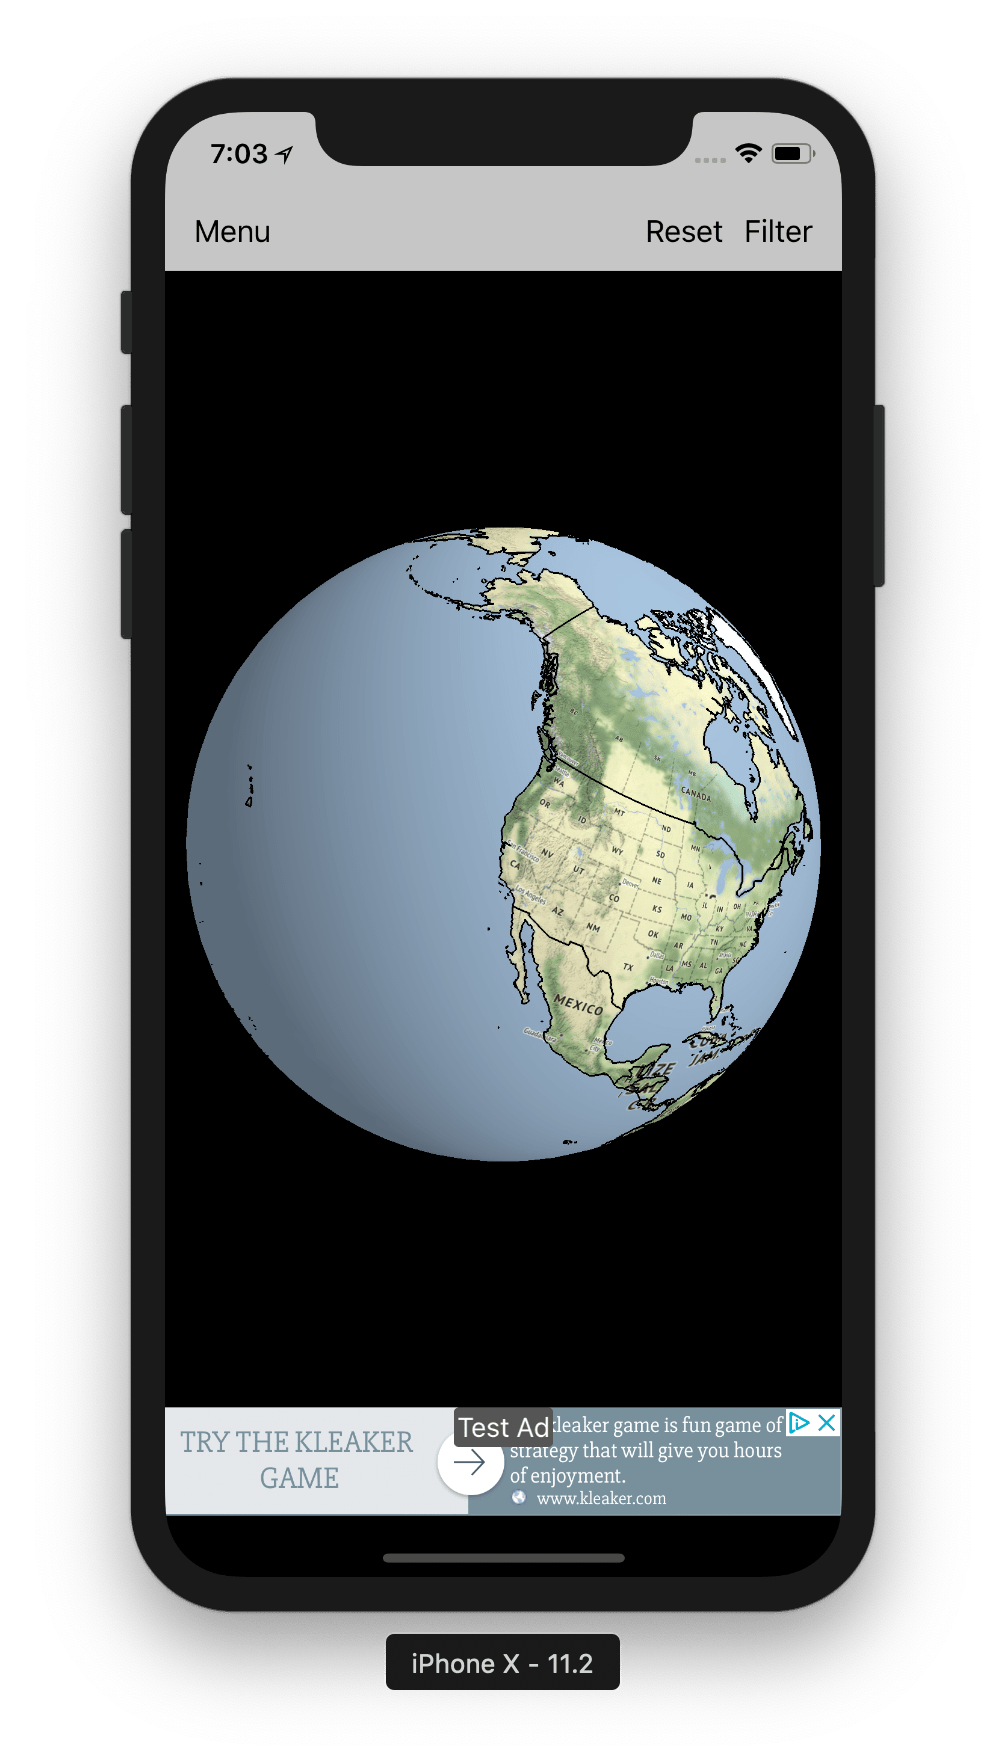
\includegraphics[width=0.8\linewidth]{figures/ch4/home_globe.png}
            \caption{NDVI selected}\label{Fig:ndvi_selected}
        \end{minipage}\hfill
        \begin{minipage}{0.5\textwidth}
            \centering
            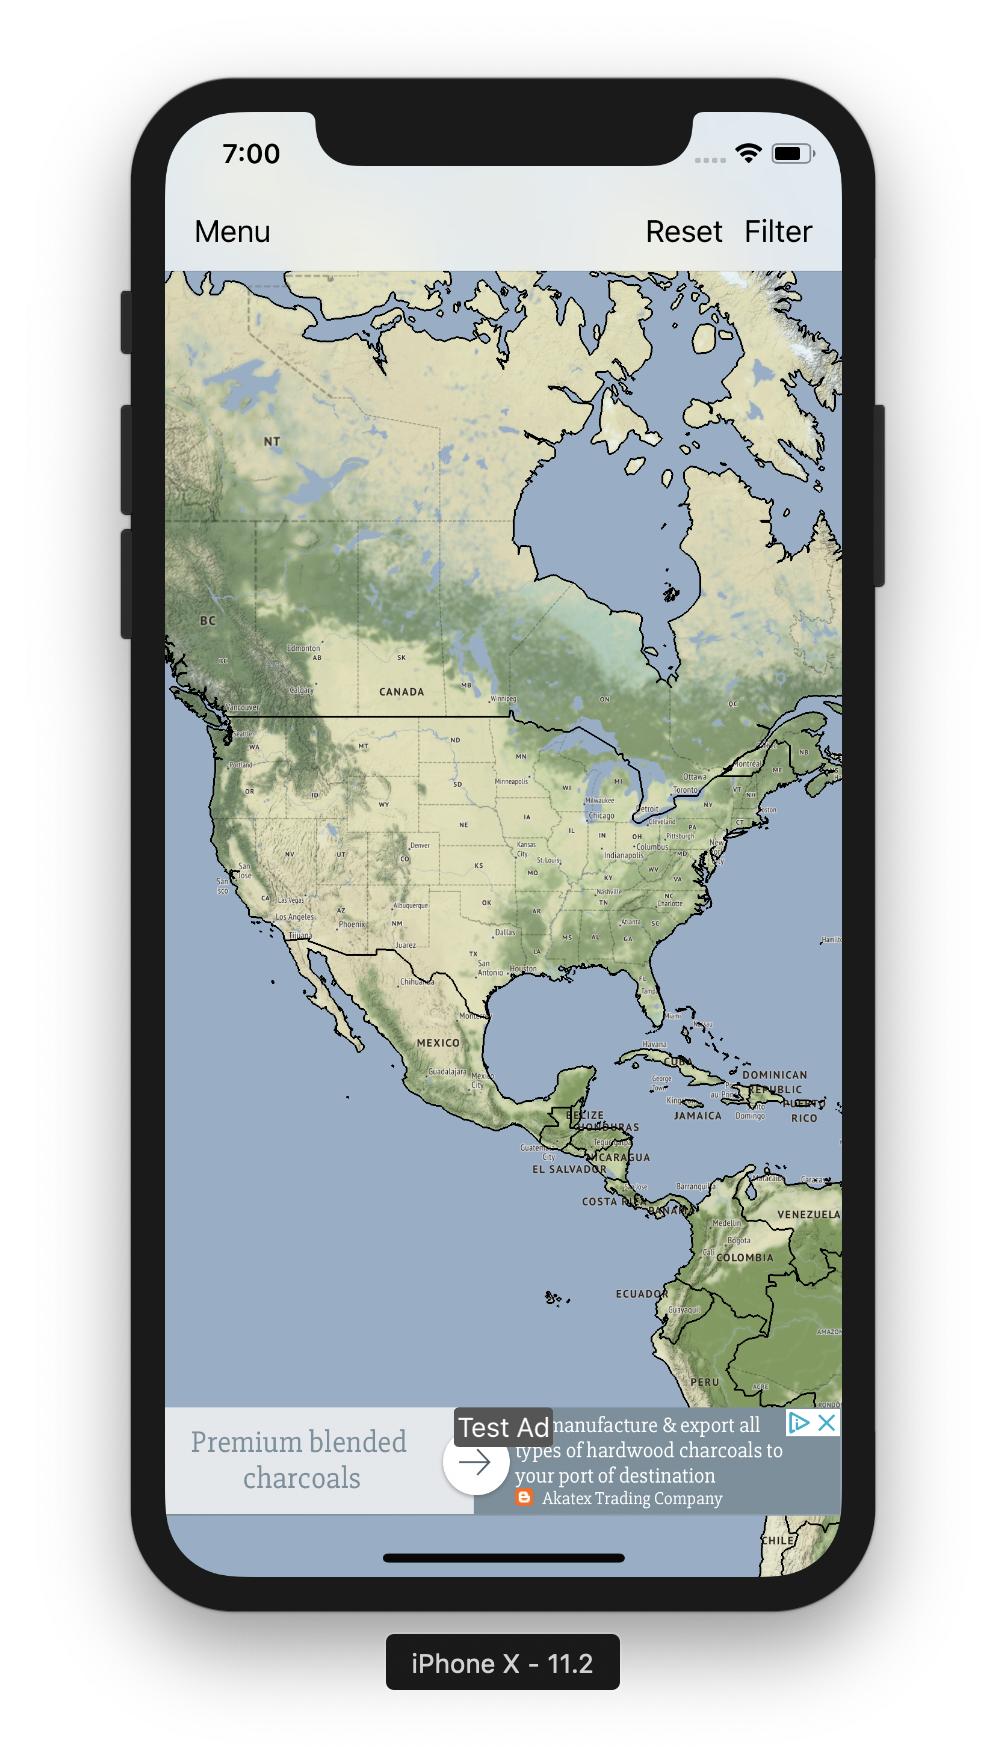
\includegraphics[width=0.8\linewidth]{figures/ch4/home.png}
            \caption{Anomaly selected}\label{Fig:anomaly_selected}
        \end{minipage}
    \end{figure}
    
    \newpage
    
    \item Globe or Map - Visualization medium
    
    User has the option to choose between 2D map view or Globe view.
    This has shown in figures 4.16 and 4.17. \\
    
    \item Year and date
    
    Year and date list is to pick a specific date for which he wants to see the data. Dates are only available after selecting the year from year list screen.
    
    Note: The year list and dates for that year is coming from server, so user will not see those dates or years which we don't have the data for.
    This dynamic thing has been done to increase user interaction and to give the stability to the app by making it dynamic as well as keeping in mind for future updates.
    
    % click year - blurr on other and show date list screen
    
    Figure 4.23 and 4.24 represents year and date list screens.
    
    \begin{figure}[!htb]
        \begin{minipage}{0.5\textwidth}
            \centering
            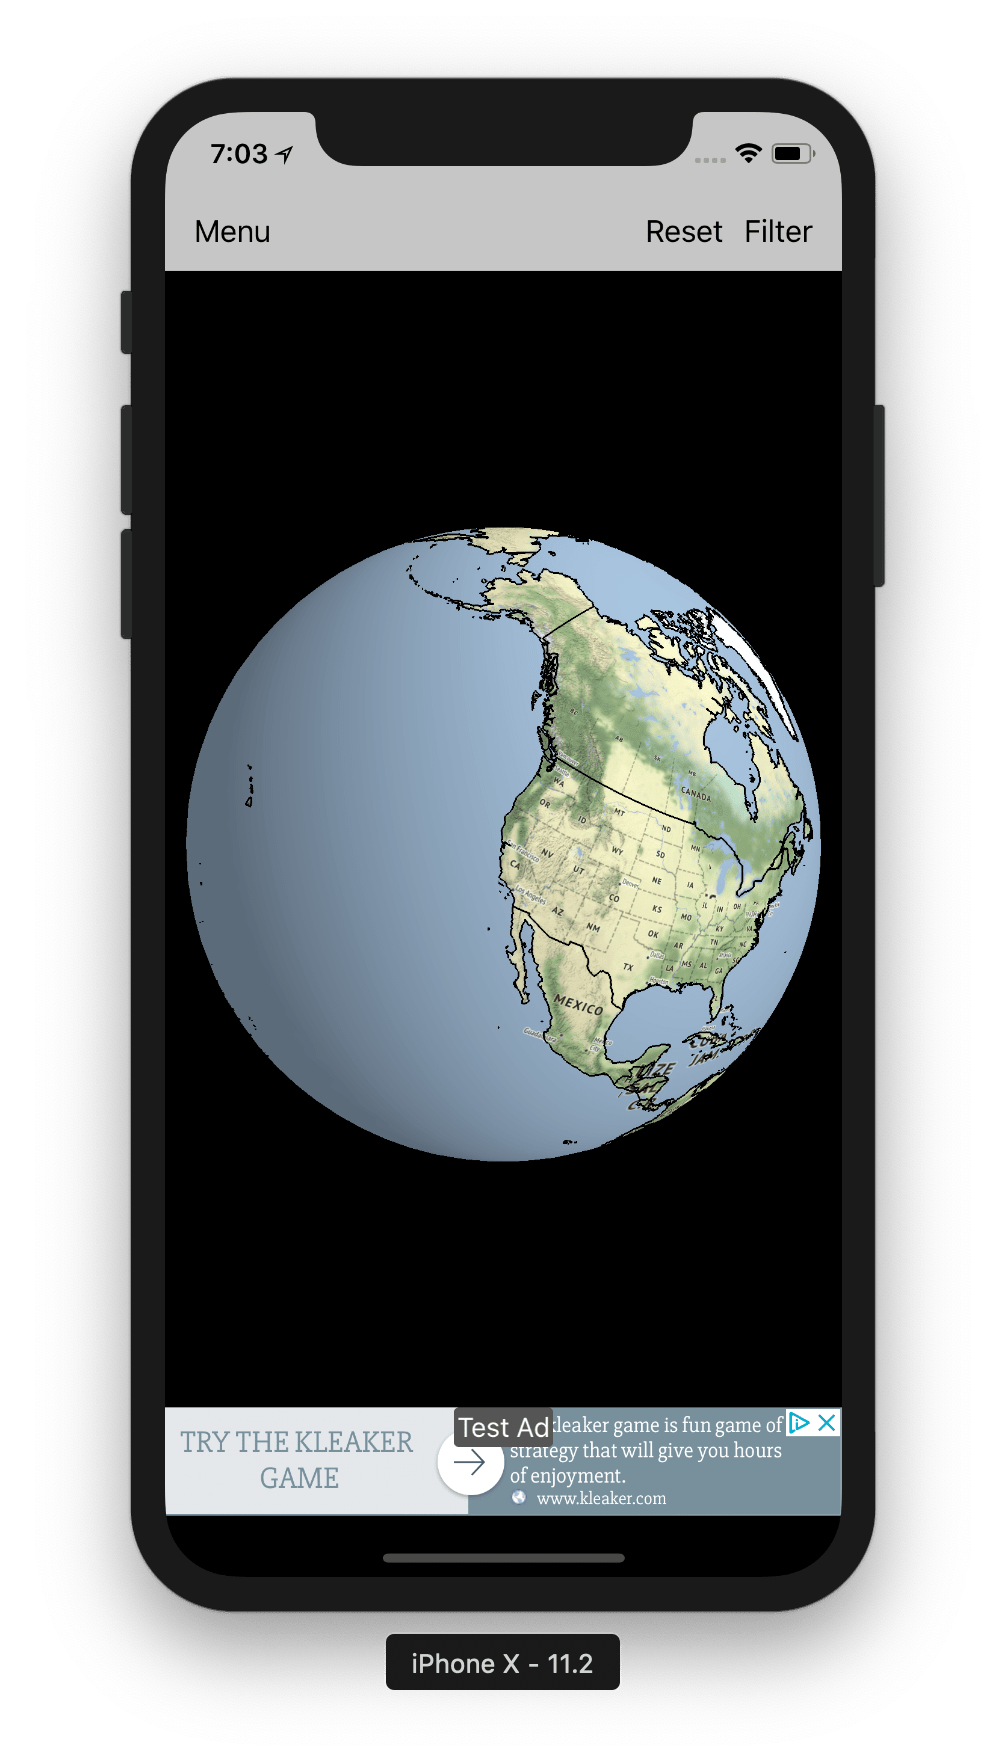
\includegraphics[width=0.8\linewidth]{figures/ch4/home_globe.png}
            \caption{NDVI selected}\label{Fig:ndvi_selected}
        \end{minipage}\hfill
        \begin{minipage}{0.5\textwidth}
            \centering
            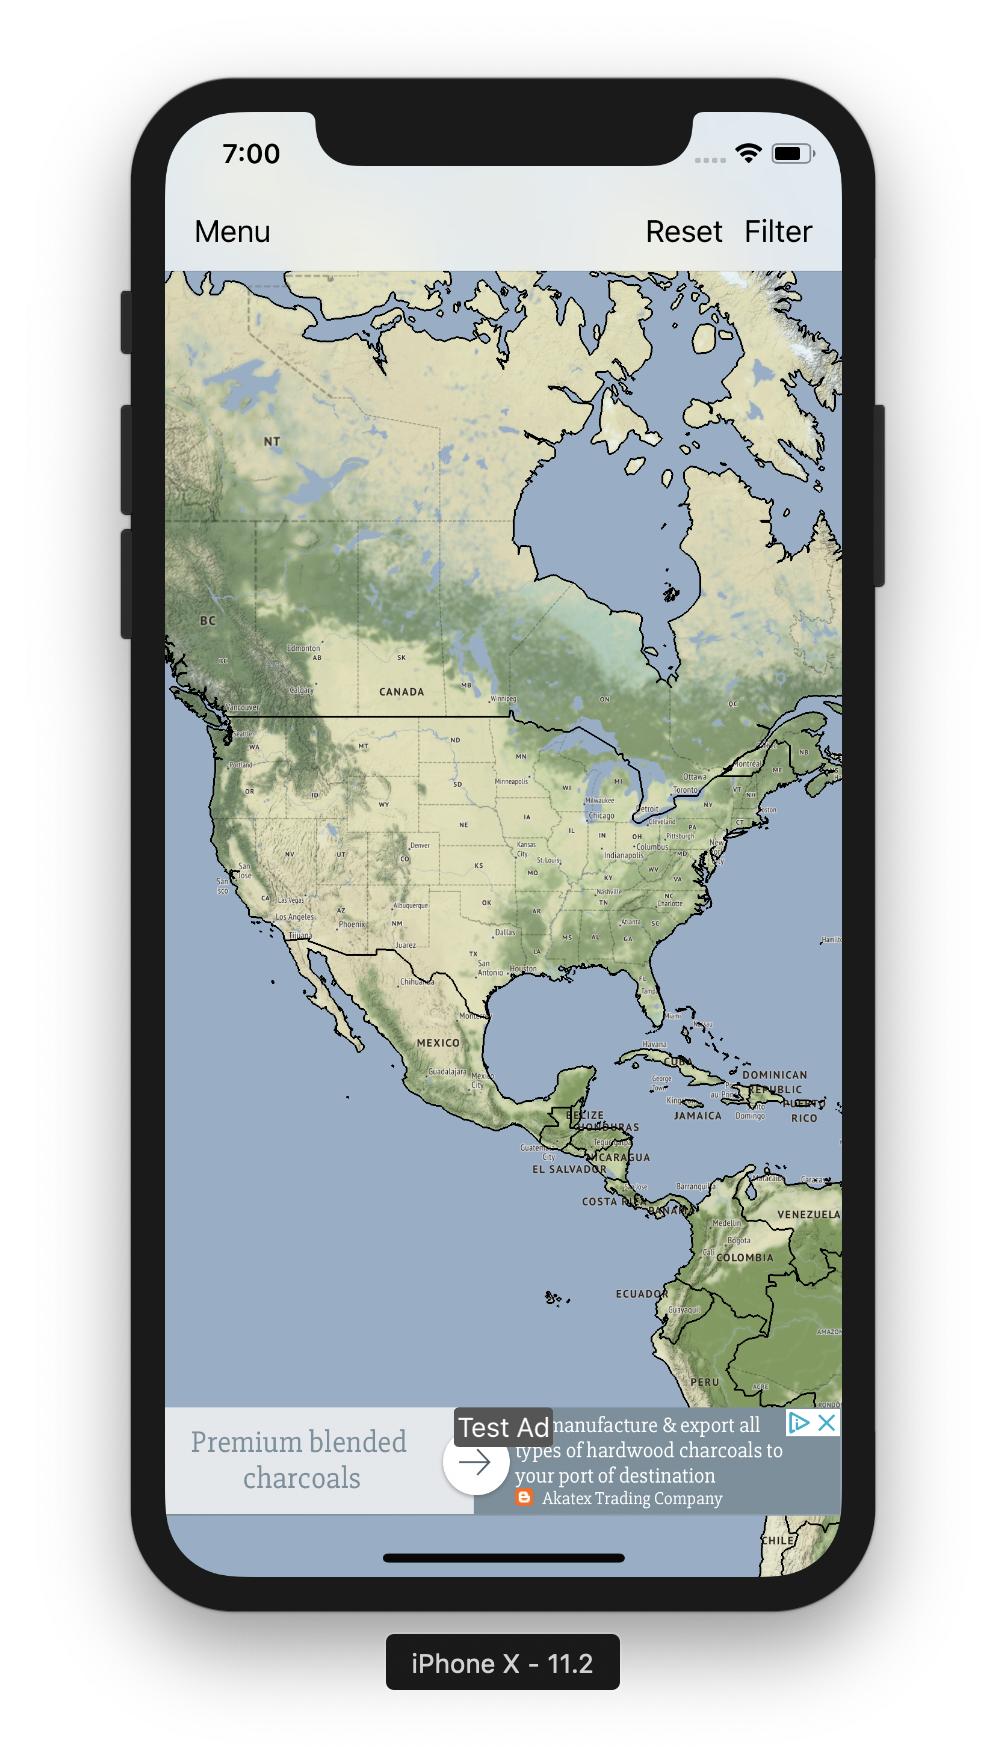
\includegraphics[width=0.8\linewidth]{figures/ch4/home.png}
            \caption{Anomaly selected}\label{Fig:anomaly_selected}
        \end{minipage}
    \end{figure}
    
    \newpage
    
    \item Color scheme
    
    %add images of color schemes used in this project too
    
    This is an additional feature which has given to the application to make it interesting. It enables user to view the data into different color palette forms.
    Remember, the color palettes are custom made and stored locally in \gls{json} files according to the \gls{ndvi} range.
    
    Figure 4.25 shows color palette options available in the app. User just have to select any of the available options and tap apply to make the commit to the choice.
    
     \begin{figure}[H]
            \centering
            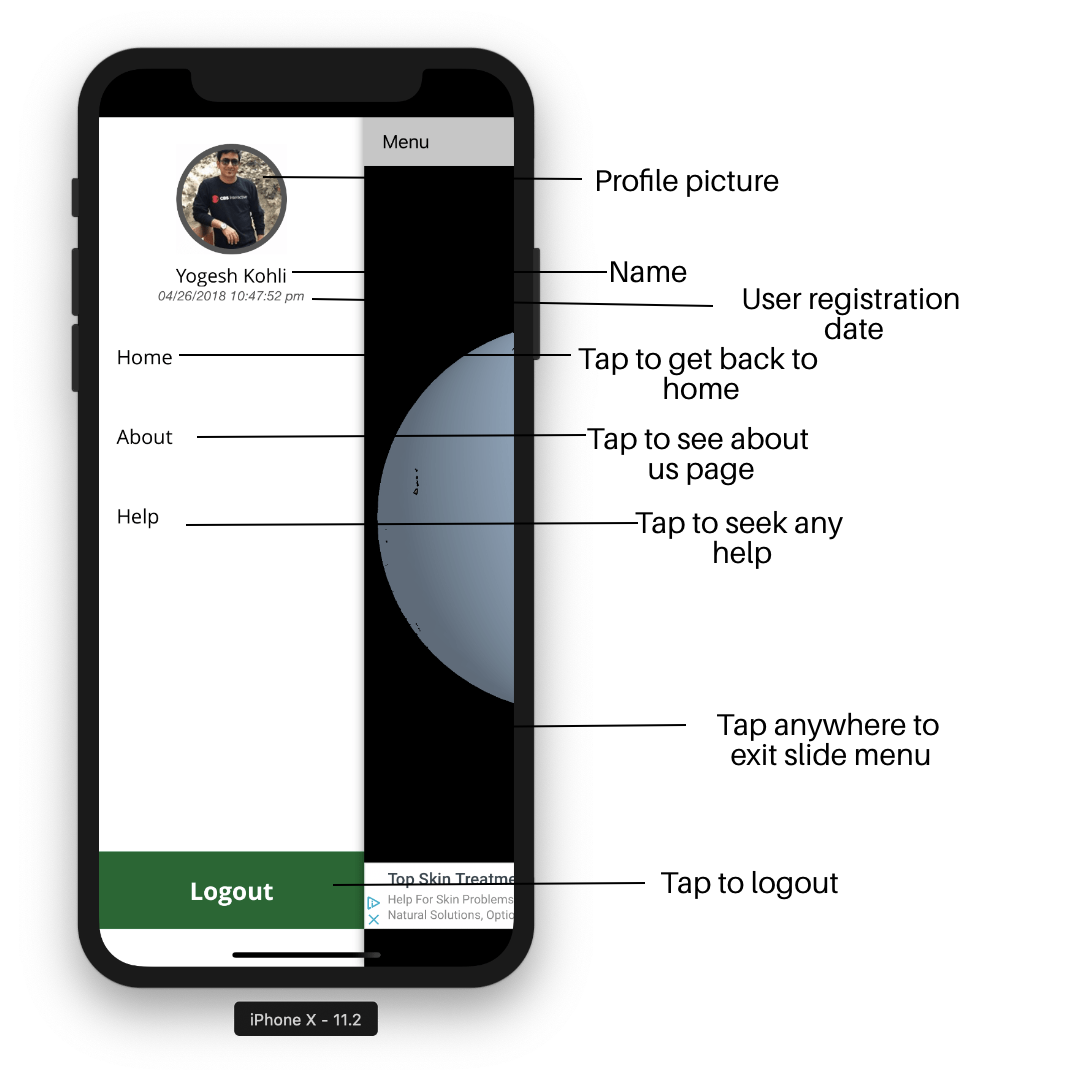
\includegraphics[width=0.35\linewidth]{figures/ch2/side_menu.png}
            \caption{\label{fig:pass_recovery_1} About us screen}
    \end{figure}
        
    Here is an example of part of one of the entries of \gls{json} file.
    
    \begin{figure}[H]
            \centering
            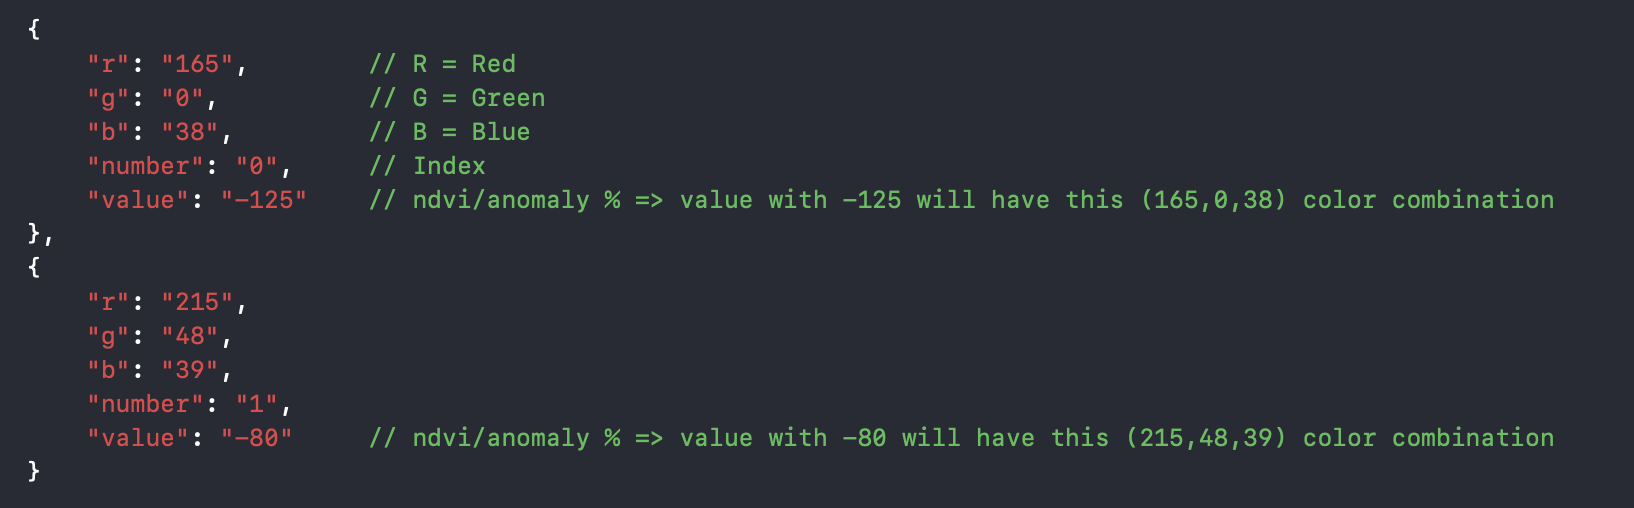
\includegraphics[width=1.0\linewidth]{figures/ch4/color_map_final.png}
            \caption{\label{fig:color_json} JSON sample of colormap file}
    \end{figure}

    \newpage
    
\end{itemize}



\section{BACK-END OF THE APP}


\subsection{Process of getting data from NASA's server}

This procedure of getting information from NASA's server and afterward putting away the information into PostgreSQL database is a significant advance in the undertaking. It involves the development of a script in Python 3.6. The data on Nasa's server is in \gls{geoTiff} format. Important thing to note here is that all the \gls{geoTiff} files that exist in their server are compressed via zip.

%put source wikipedia here

According to Wikipedia, \gls{geoTiff} is a public domain metadata standard which allows georeferencing information to be embedded within a TIFF file. The potential additional information includes map projection, coordinate systems, ellipsoids, datums, and everything else necessary to establish the exact spatial reference for the file.

Figure 4.27 represents NASA's data bundled in \gls{geoTiff} file.

    \begin{figure}[H]
            \centering
            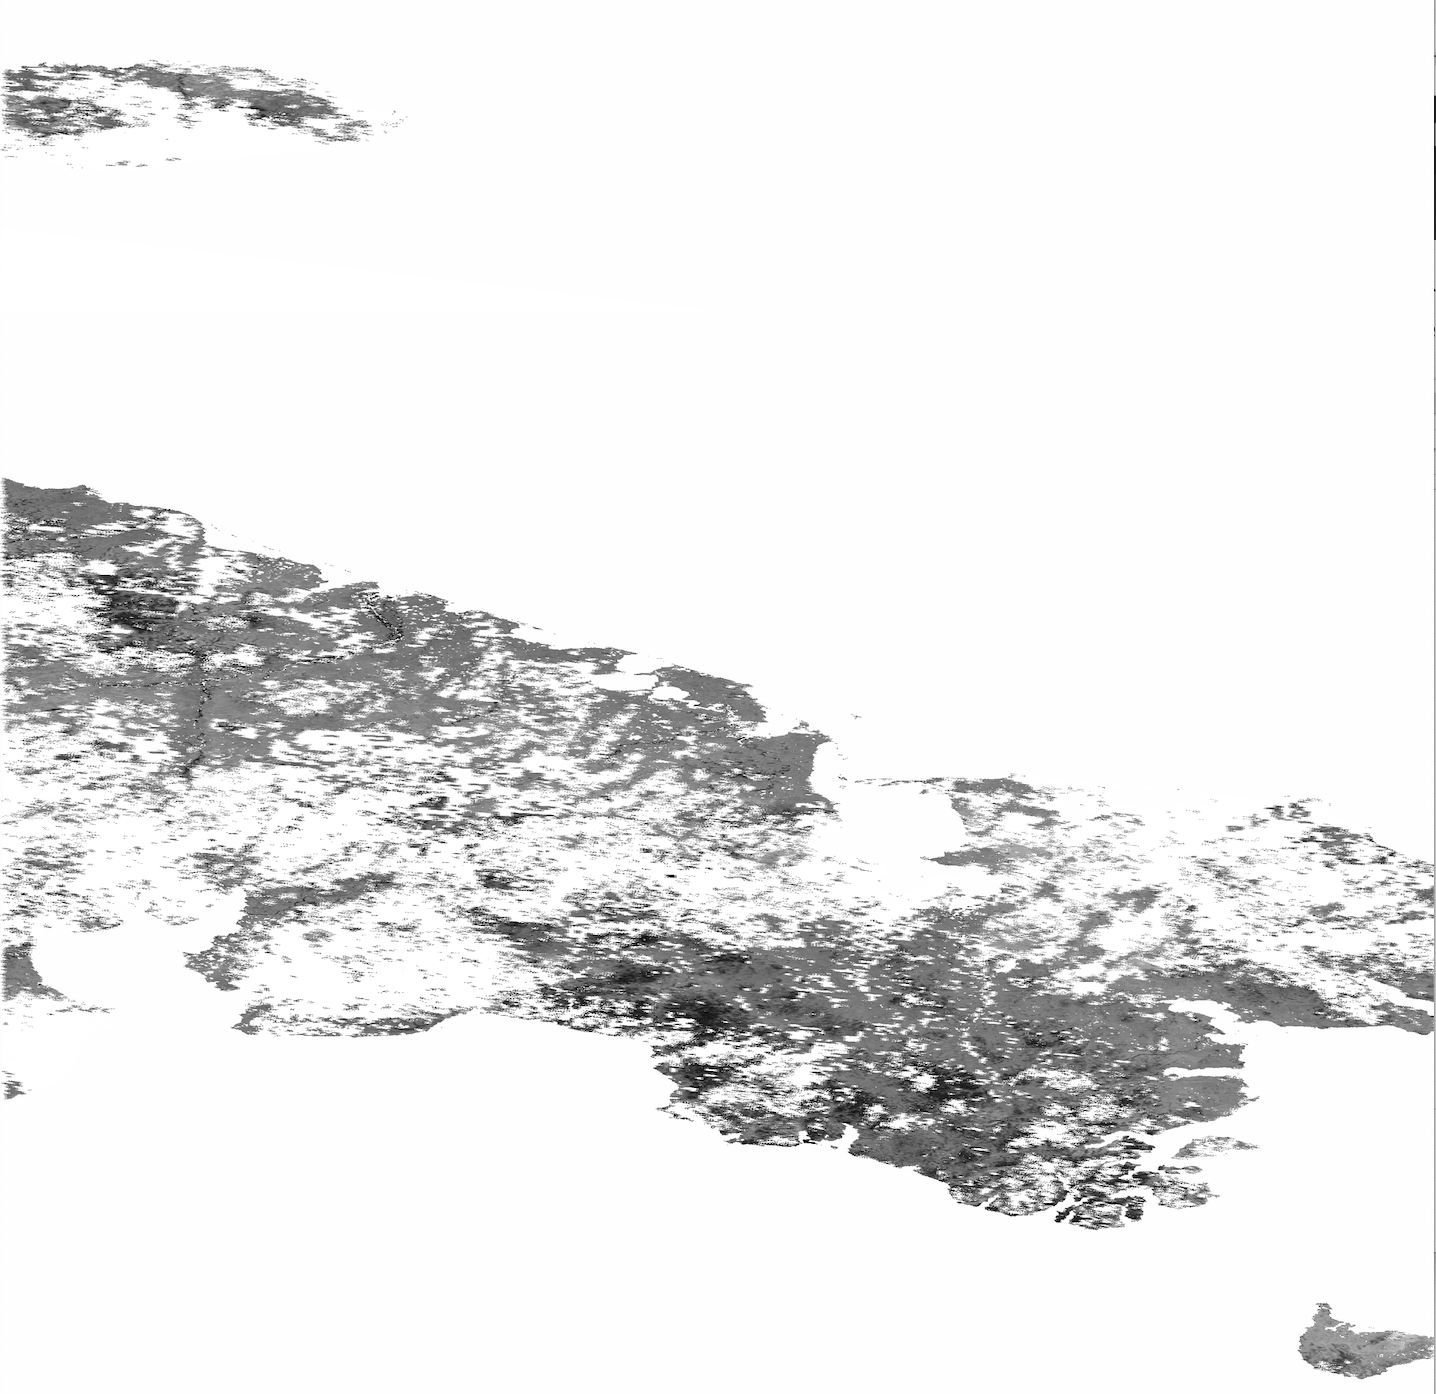
\includegraphics[width=0.35\linewidth]{figures/ch4/geotiff.png}
            \caption{\label{fig:geotiff} Sample of NASA's NDVI Data file}
    \end{figure}

    Steps taken to get the raw data from this \gls{geoTiff} file, process the data and finally to store that data to a database are as follows :-
    
    \begin{itemize}
        \item Find the beginning of the 8-day set and make your string formatted according to Nasa's file name format.
        
        \item Open zip without unfastening it in such a case that you unfasten the file, the record gets 16 times bigger in size which at last puts weight on processor to process the file.
        
        \item Read the file row by row one at a time and process the data accordingly by converting data points to \gls{ndvi} values.
        
        \item Customizing the data according to the database structure and finally storing that data there.
    \end{itemize}

\subsection{Web services required for JSON parsing between database and the front-end}

% https://docs.oracle.com/javaee/6/tutorial/doc/gijqy.html

\textbf{RESTful web services} are built to work best on the Web. Representational State Transfer (REST) is an architectural style that specifies constraints, such as the uniform interface, that if applied to a web service induce desirable properties, such as performance, scalability, and modifiability, that enable services to work best on the Web. In the REST architectural style, data and functionality are considered resources and are accessed using Uniform Resource Identifiers (URIs), typically links on the Web. The resources are acted upon by using a set of simple, well-defined operations. The REST architectural style constrains an architecture to a client/server architecture and is designed to use a stateless communication protocol, typically HTTP. In the REST architecture style, clients and servers exchange representations of resources by using a standardized interface and protocol. \\

\textbf{\gls{json}} is a lightweight information trade arrange. JSON is a content arrangement that is totally dialect free yet utilizes traditions that are recognizable to software engineers of the C-group of dialects, including C, C++, Java, JavaScript, PHP, Python, and numerous others. These properties make JSON a perfect information exchange dialect and helps developers to transfer data between the server and the front-end of any software. The language used for creating web services is \textbf{\gls{php}}. \\

List of web services creates for the project :-

\begin{itemize}
    \item \textbf{dbcon.php} \\
    It contains a database connection function for connecting to PostgreSQL database. \textbf{pg\_connect} function has been used to connect to the database. It opens up a connection to the database specified by the credentials of the server in the connection string. \\
    
    \item \textbf{credentials.php} \\
    It contains all the services related to login, register and forgot password. \\
    
    \item \textbf{getdata.php} \\
    It has all the services for the ndvi data including filtering process. \\
\end{itemize}

\newpage

\section{USING THE APP}

\subsection{Data Visualization}

%this section will include images of the home screen different cases and explaining that images

% have some info about the image - date selected, country selected, mean values and all and show them in the picture

This section contains all three cases of Admin Level and their effect on Home screen i.e data visualization. \\

Different types of level data are :-

\begin{itemize}
    \item \textbf{Admin Level 0 - Country Wise} \\
    The country has been colored with value of mean for the whole country on particular date calculated using the appropriate formulae. \\
    
     \begin{figure}[H]
            \centering
            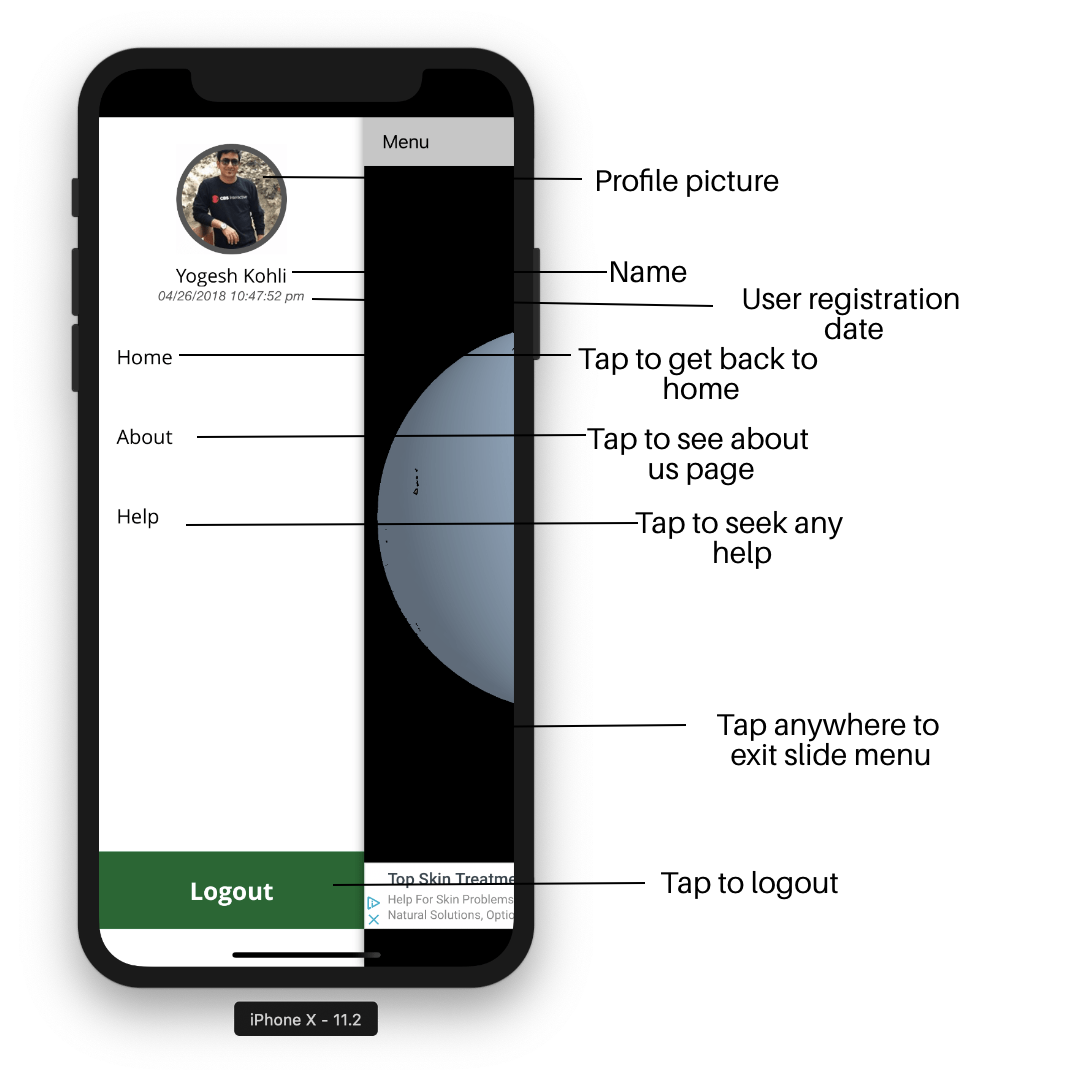
\includegraphics[width=0.5\linewidth]{figures/ch2/side_menu.png}
            \caption{\label{fig:pass_recovery_1} About us screen}
        \end{figure}
    
    \newpage
    
    \item \textbf{Admin Level 1 - State Wise} \\
    Mean for every state under specific country for specific date has been calculated and colored accordingly. \\
    
    \begin{figure}[H]
            \centering
            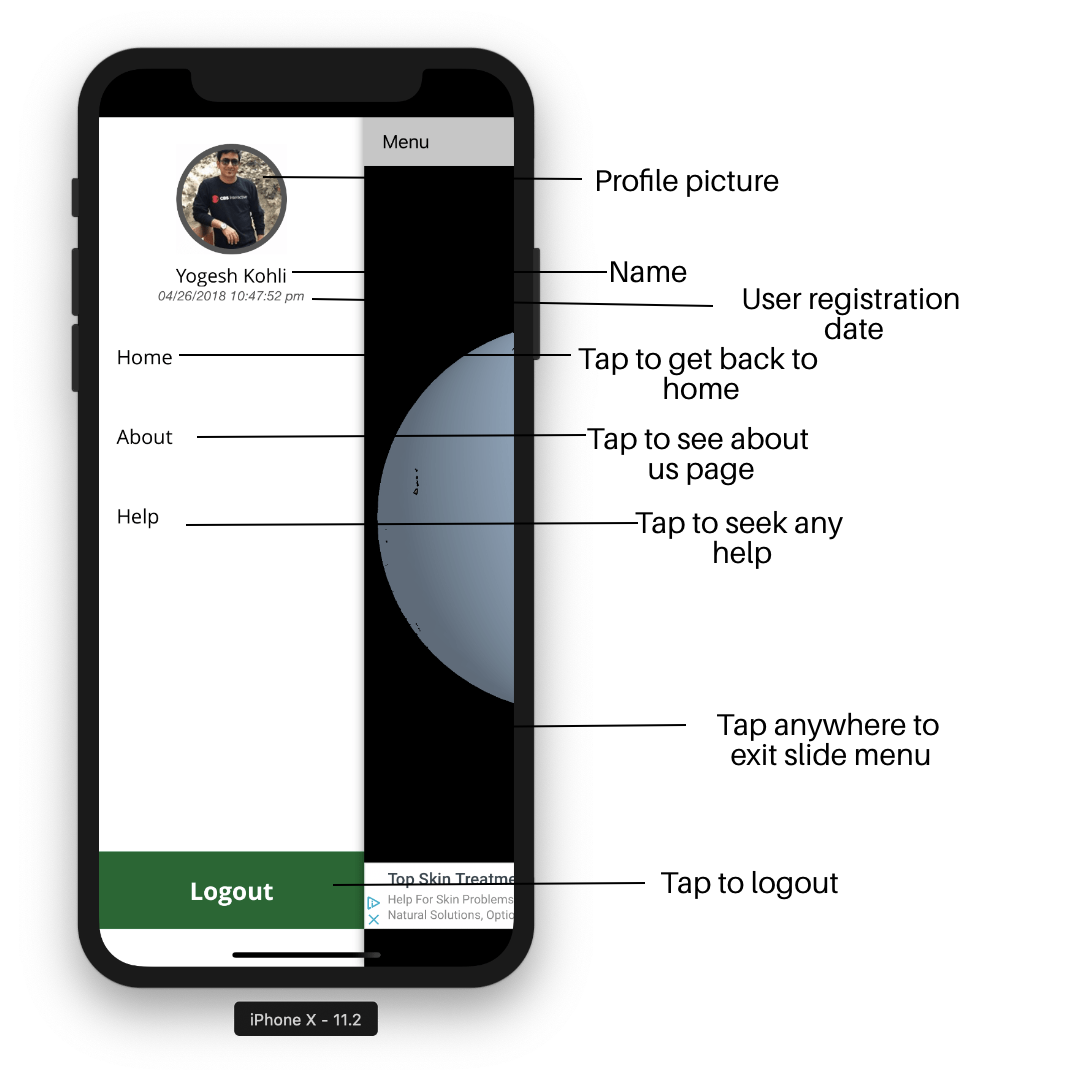
\includegraphics[width=0.5\linewidth]{figures/ch2/side_menu.png}
            \caption{\label{fig:pass_recovery_1} About us screen}
        \end{figure}
    
    \newpage
    
    \item \textbf{Admin Level 2 - District Wise} \\
    District mean values has been calculated for the country and then district regions have been colored accordingly. \\
    
     \begin{figure}[H]
            \centering
            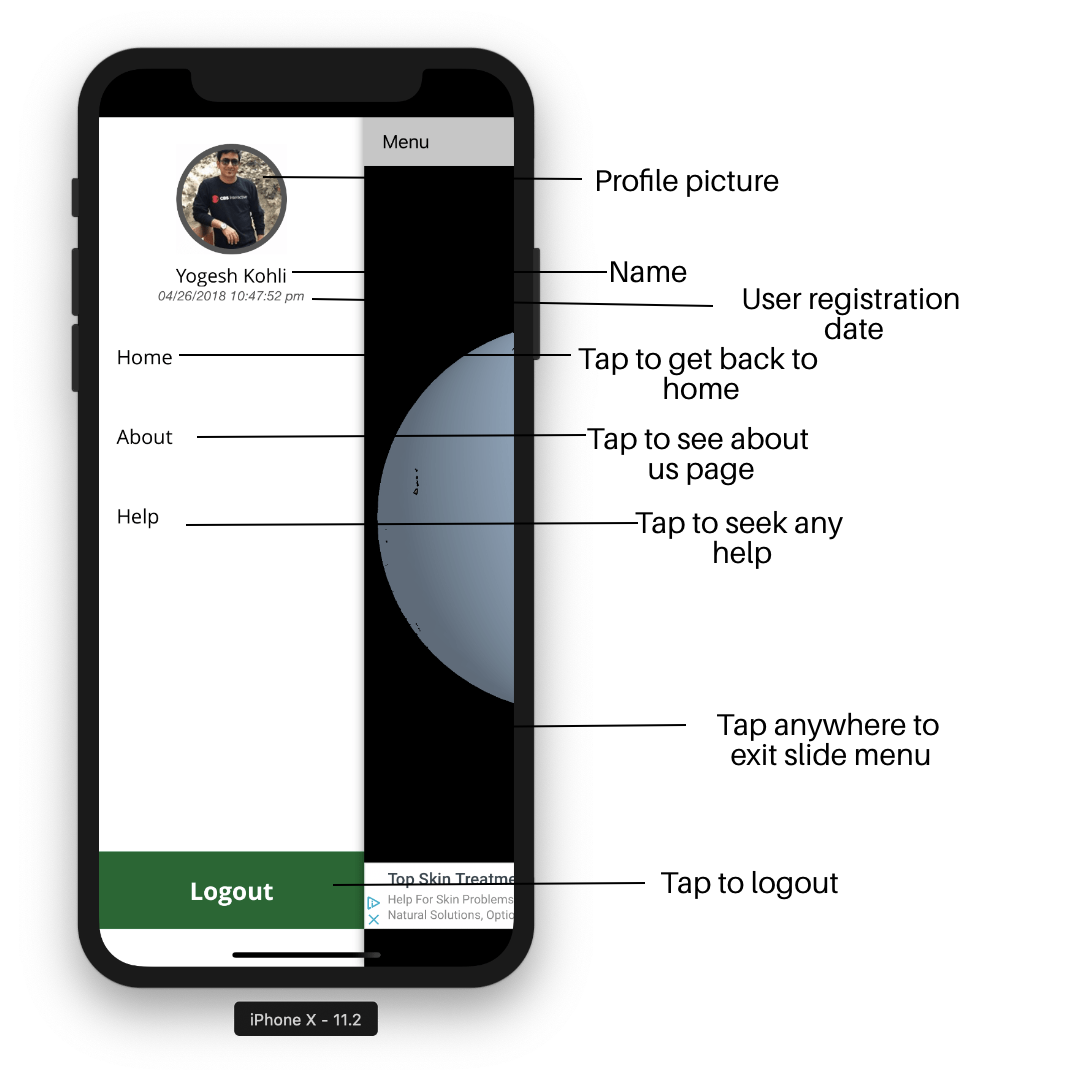
\includegraphics[width=0.5\linewidth]{figures/ch2/side_menu.png}
            \caption{\label{fig:pass_recovery_1} About us screen}
        \end{figure}
    
\end{itemize}

\newpage


\section{APIs, Softwares, Design pattern and Languages Usage}

\subsection{APIs Usage}

Major APIs used in the project to make the application better are:-

\begin{itemize}
    \item \textbf{Alamofire} - HTTP Networking Library
    
    Alamofire is a Swift-based HTTP networking library for \gls{iOS} and \gls{macOS}. It gives a rich interface over Apple's Foundation organizing stack that disentangles various basic networking assignments.\\
    
    It can be found here - \url{https://github.com/Alamofire/Alamofire} \\
   
    \item \textbf{WhirlyGlobe} - Globe SDK
    
    Focusing on mobile technology with based on OpenGL ES, WhirlyGlobe-Maply is an open source library which is utilized in a wide assortment of Atlas, climate, representation, and guide applications. The \gls{sdk} is both a 3D intelligent globe for \gls{iOS} and a 2D map for \gls{iOS}. \\
    
    One important thing to mention is this library has been customized a lot according to the needs of the application. Classes has been modified by adding some delegate methods which enables developers to have more control on the visualization. \\
    
    It can be found here - \url{https://github.com/mousebird/WhirlyGlobe} \\
    
    \item \textbf{SwiftCSVExport} - Exporting data
    
    Swift CSV Export is lightweight and rich highlights framework and it accommodating to make, read and compose CSV records in basic way. \\
    
    This library has been utilized to change over the JSONDictionary to the required objects which it takes and to package the information into CSV file and at last to send out it through email. Remember, this library has also been customized and used according to our data types requirements. \\
    
    It can be found here - \url{https://github.com/vigneshuvi/SwiftCSVExport} \\ 
    
\end{itemize}

\newpage

\subsection{Softwares used in the project}

List of Softwares used in the project with their significance are :-

\begin{itemize}
    \item \textbf{Xcode}
    It's an \gls{ide} by Apple and is used for development of the app. \\
    
    \item \textbf{Axure RP 8}
    Used for creating wireframes \\
    
    \item \textbf{Bracket}
    It's a text editor used to code web services in \gls{php}. \\
    
    \item \textbf{FileZilla}
    It's a cross platform \gls{ftp} application used to update and transfer files to server. \\
    
\end{itemize}


\subsection{Design Pattern used}

%biblipgraphy - https://developer.mozilla.org/en-US/docs/Web/Apps/Fundamentals/Modern_web_app_architecture/MVC_architecture

\textbf{\gls{mvc}} is a software architecture pattern, commonly used to implement user interfaces: it is therefore a popular choice for architecting web apps. In general, it separates out the application logic into three separate parts, promoting modularity and ease of collaboration and reuse. It also makes applications more flexible and welcoming to iterations. \\

%bibliography https://developer.apple.com/library/archive/documentation/General/Conceptual/DevPedia-CocoaCore/MVC.html

According to Apple's documentation about design patterns, \gls{mvc} is central to a good design for a Cocoa application. The benefits of adopting this pattern are numerous. Many objects in these applications tend to be more reusable, and their interfaces tend to be better defined. Applications having an \gls{mvc} design are also more easily extensible than other applications. Moreover, many Cocoa technologies and architectures are based on \gls{mvc} and require that your custom objects play one of the \gls{mvc} roles. \\



%talk about MVC architecture used
%singleton used
%key value observer - notifications

As explained in the definition, MVC is as direct as its name. It's comprised of three layers: the model, the view and the controller.

\begin{itemize}
    \item \textbf{Model} \\
    The Model is the place your data lives. Things like parsers and networking code typically live there. \\
    
    \item \textbf{View} \\
    The View layer is the essence of your application. Its classes are commonly reusable, since there aren't any area particular rationale in them. For instance, a UILabel is a view that presents message on the screen, and it's effectively reusable. \\
    
    \newpage
    
    \item \textbf{Controller} \\
    The Controller intercedes between the view and the model, normally through the delegation concept. In the perfect situation, the controller element won't know the solid view it's managing. Rather, it will speak with an abstraction with the help of protocols. An exemplary model is the manner in which a UITableView interacts with its data source through the UITableViewDataSource protocol. \\
    
\end{itemize}


\gls{mvc} has been shown visually in the figure 4.31.

    \begin{figure}[H]
            \centering
            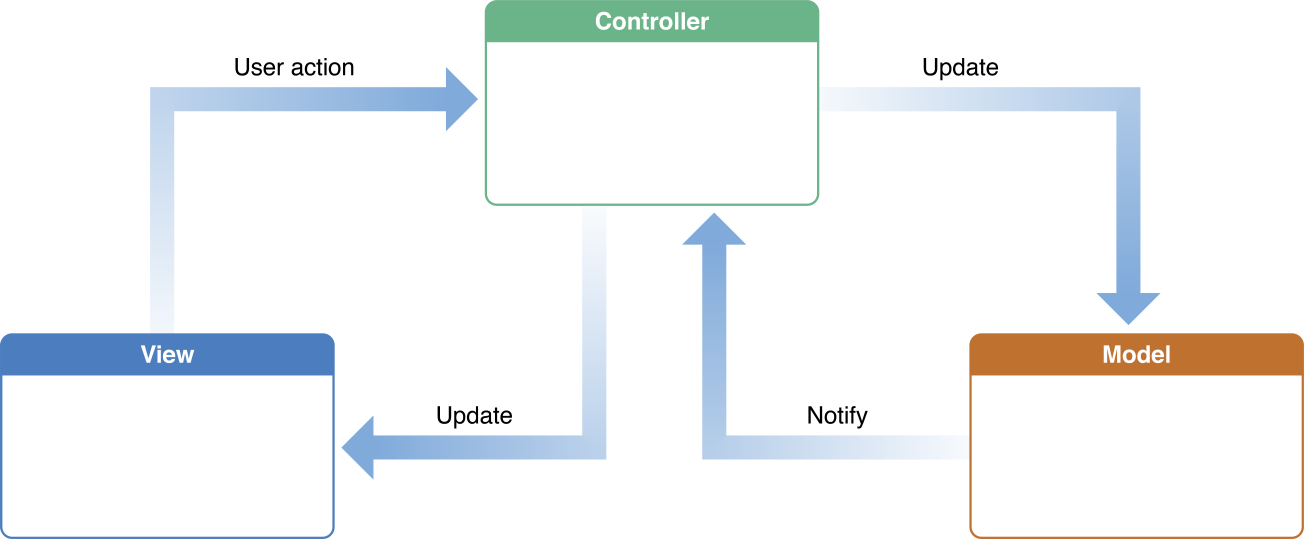
\includegraphics[width=1.0\linewidth]{figures/ch4/mvc.png}
            \caption{\label{fig:mvc} MVC Architecture}
        \end{figure}

\subsection{Software Languages used in the project}

List of software languages used in the process :-

\begin{itemize}
    \item \textbf{Swift 4.1} - for development of iOS app \\
    \item \textbf{PHP} - for data parsing between server and the app \\
    \item \textbf{Python} - script for getting data from \gls{nasa}'s server and storing it in database. \\
\end{itemize}
